%versi 2 (8-10-2016)
\lstset{
  basicstyle=\ttfamily,
  columns=fullflexible,
  frame=single,
  breaklines=true,
  showlines=true,
  postbreak=\mbox{\textcolor{red}{$\hookrightarrow$}\space},
}

\chapter{Landasan Teori}
\label{chap:teori}
\setcounter{secnumdepth}{3}
%Pada bab ini dijelaskan dasar-dasar teori mengenai \textit{BlueTape}, \textit{Heroku}, \textit{PostgreSQL}, \textit{GMail}, dan \textit{Line@}.



%2.1 BlueTape
\section{BlueTape}
\label{sec:BlueTape}
BlueTape adalah aplikasi yang berfungsi untuk membantu urusan-urusan \textit{paper-based} di FTIS UNPAR menjadi \textit{paperless}. Aplikasi ini berbasis web dengan memanfaatkan \textit{framework} CodeIgniter dan ZURB Foundation. Selain itu, BlueTape menggunakan layanan OAuth dari Google untuk autentikasi pengguna. Saat skripsi ini ditulis, aplikasi BlueTape memiliki tiga layanan, yaitu Transkrip \textit{Request} / \textit{Manage}, Perubahan Kuliah \textit{Request} / \textit{Manage}, dan perekam jadwal dosen. Layanan Transkrip \textit{Request} / \textit{Manage} memberikan layanan untuk melakukan permohonan serta pencetakan transkrip mahasiswa. Layanan Perubahan Kuliah \textit{Request} / \textit{Manage} memberikan layanan untuk permohonan dan pencetakan perubahan jadwal kuliah oleh dosen. Layanan perekam jadwal dosen memberikan layanan untuk menyimpan dan menampilkan jadwal dosen. \footnotemark
\footnotetext{https://github.com/ftisunpar/BlueTape}


%2.2 Heroku
\section{Heroku ~\cite{heroku}}
\label{sec:Heroku}
Heroku adalah \textit{cloud platform} yang memungkinkan \textit{developer} untuk membangun, menjalankan, dan mengoperasikan aplikasi pada \textit{cloud}. Heroku mendukung beberapa bahasa pemrograman, meliputi : Ruby, Node.js, Java, Python, Clojure, Scala, Go, dan PHP.

\subsection{Arsitektur Heroku}
Heroku memungkinkan seorang \textit{developer} untuk melakukan \textit{deploy} (menyebarkan), \textit{run} (menjalankan), dan \textit{manage} (mengelola) pada aplikasi yang ditulis di dalam bahasa yang didukung oleh Heroku. Heroku mendefinisikan aplikasi sebagai gabungan dari \textit{source code} yang ditulis di dalam salah satu bahasa yang didukung Heroku, deskripsi \textit{dependency} yang dipakai, dan Procfile.

\subsubsection{\textit{Dependency}}
\textit{Developer} perlu mendeskripsikan \textit{dependency} tambahan yang diperlukan agar aplikasi dapat dibangun dan dijalankan. Aturan penulisan deskripsi \textit{dependency} berbeda-beda untuk tiap bahasa. Contoh : pada aplikasi dengan bahasa Node.js, deskripsi \textit{dependency} ditulis di dokumen \texttt{package.json}.

\subsubsection{Procfile}
\textit{Developer} perlu memberitahu Heroku bagian aplikasi yang dapat dijalankan. Jika \textit{developer} menggunakan framework yang sudah ada, Heroku dapat mencari tahu. Contoh : pada aplikasi dengan bahasa Node.js, Heroku dapat mengetahui bagian aplikasi yang dijalankan pada bagian \texttt{main} di dalam \texttt{package.json}. Untuk aplikasi lain, \textit{developer} mungkin perlu menyatakan apa yang harus dieksekusi secara eksplisit. Caranya dengan menyertakan sebuah dokumen teks bernama Procfile. 

Dokumen Procfile tidak memiliki ekstensi dokumen, seperti \texttt{.txt}, \texttt{.docx}, \texttt{.jpg} dan lain-lain. Apabila Procfile diberi ekstensi dokumen (contoh : Procfile.txt), maka Procfile tersebut tidak sah. Selain itu, Procfile harus diletakkan di direktori \texttt{root}. Jika diletakkan di tempat lain, Procfile tidak akan berfungsi sebagaimana mestinya.

Isi dari Procfile adalah satu atau lebih baris yang menyatakan \textit{process type}. Format penulisan tiap baris Procfile adalah : 
\begin{lstlisting}

	<process type>: <command>

\end{lstlisting}
Keterangan :
\begin{itemize}
\item \texttt{<process type>} : nama perintah yang mengandung huruf dan angka. Contoh : \texttt{web}, \texttt{worker}, \texttt{urgentworker}, \texttt{clock}, dan lain-lain. Untuk aplikasi sederhana, \textit{developer} cukup menuliskan \textit{process type} \texttt{web} saja.
\item \texttt{<command>} : perintah yang harus dijalankan oleh setiap dyno dari \textit{process type} tersebut pada saat startup.
\end{itemize}
 
Contoh isi Procfile :
\begin{lstlisting}

	web: java -jar lib/foobar.jar \textdollar PORT

\end{lstlisting}

Pada contoh, \texttt{web} merupakan \texttt{<process type>}, sedangkan \texttt{web: java -jar lib/foobar.jar \textdollar PORT} adalah perintah yang harus dijalankan agar \textit{process type} tersebut berjalan. Perintah tersebut berfungsi untuk menyalakan web server.

Procfile tidak wajib dibuat untuk sebagian besar bahasa pemrograman yang didukung Heroku. Heroku akan secara otomatis mendeteksi bahasa yang digunakan, dan membuat \textit{process type} \texttt{web} untuk menjalankan server aplikasi. Apabila aplikasi menggunakan \texttt{heroku.yml} sebagai \textit{build manifest}, Procfile juga tidak diwajibkan. Perintah yang disebutkan di bagian \texttt{run} pada \texttt{heroku.yml} harus mengikuti format yang sama dengan format Procfile (kecuali \textit{process type} \textit{release}).


\subsubsection{\textit{Process Type}}
Ada tiga kelompok \textit{process type} : 
\begin{itemize}
\item \textit{process type} \texttt{web}
\item \textit{process type} \texttt{worker} : \textit{process type} apapun selain \texttt{web}
\item \textit{process type} \texttt{singleton} : \textit{process type} yang bersifat sementara dan dapat berjalan terpisah
\end{itemize}

Di antara beragam \textit{process type}, ada dua \textit{process type} spesial : \textit{process type} \texttt{web} dan \texttt{release}. \textit{Process type} \texttt{web} adalah satu-satunya \textit{process type} yang dapat menerima arus HTTP eksternal dari router Heroku. Jika sebuah aplikasi melibatkan \textit{web server}, \textit{developer} harus menyatakannya sebagai proses \texttt{web}. \textit{Process type} \texttt{release} adalah \textit{process type} yang digunakan untuk menyebutkan perintah yang dijalankan selama fase release.

\begin{figure}[H]
	\centering  
	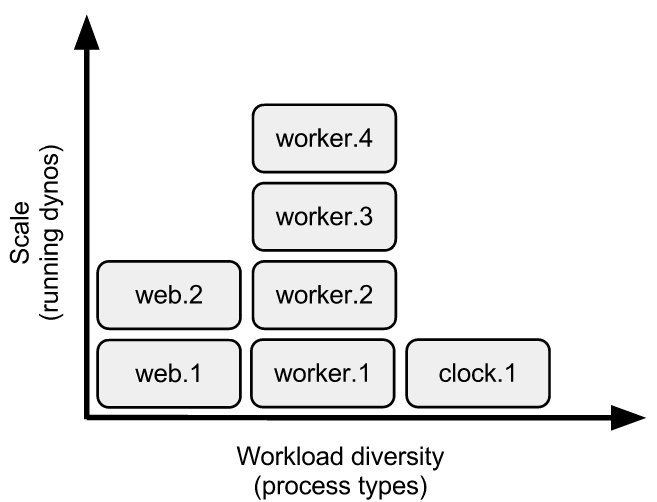
\includegraphics[scale=0.5]{process-type-dyno-relationship.jpg}  
	\caption[Diagram hubungan antara \textit{process type} dan dyno]{Diagram hubungan antara \textit{process type} dan dyno} 
	\label{fig:process-type-dyno-relationship} 
\end{figure}

\textit{Process type} dan dyno saling berhubungan. \textit{Process type} adalah prototipe yang menjadi tempat dimana dyno dibentuk. Hubungan \textit{process type} dan dyno dapat dilihat di diagram pada Gambar~\ref{fig:process-type-dyno-relationship}. Sumbu x menyatakan \textit{process type} yang dipakai, sementara sumbu y menyatakan jumlah dyno yang berjalan pada \textit{process type} tersebut. Semakin banyak dyno pada suatu \textit{process type} maka konkurensi untuk pekerjaan yang ditangani \textit{process type} tersebut akan meningkat. Semakin banyak \textit{process type} maka semakin beragam beban kerja.

Untuk mengatur berapa banyak dyno yang bekerja di satu \textit{process type}, perintah yang dapat diketikkan pada command shell adalah :
\begin{lstlisting}

	$ heroku ps:scale <process=dyno list>
	
\end{lstlisting}
Keterangan :
\begin{itemize}
\item \texttt{<process=dyno list>} : daftar pasangan \textit{process type} dengan jumlah dyno yang ditugaskan untuk proses tersebut.
\end{itemize}

Contoh : 
\begin{lstlisting}

	$ heroku ps:scale web=2 worker=4 clock=1
	
\end{lstlisting}

Selain dapat mengatur jumlah dyno yang ditugaskan pada suatu pekerjaan, \textit{developer} dapat menjadwalkan proses yang berjalan pada suatu waktu atau jangka waktu tertentu. Caranya dengan menggunakan add-on Heroku Scheduler atau menggunakan \textit{process type} khusus untuk mengatur jadwal pekerjaan.

\subsubsection{Dyno}
Dyno adalah wadah aplikasi berbasis Unix yang terisolasi, tervirtualisasi, dan menyediakan lingkungan yang dibutuhkan untuk menjalankan suatu aplikasi. Umumnya, jika aplikasi di-\textit{deploy} ke Heroku untuk pertama kali, Heroku akan menjalankan satu web dyno secara otomatis.

Setiap dyno termasuk dalam salah satu dari konfigurasi berikut :
\begin{itemize}
\item Web dyno

Web dyno adalah dyno dari \textit{process type} \texttt{web} yang disebutkan di dalam Procfile. Web dyno adalah satu-satunya dyno yang dapat menerima arus HTTP dari router Heroku.

\item Worker dyno

Worker dyno adalah dyno dari \textit{process type} apapun selain \texttt{web} yang disebutkan di dalam Procfile. Worker dyno biasanya digunakan untuk pekerjaan di latar belakang, sistem antrian, dan pekerjaan yang memiliki jangka waktu.

\item One-off dyno

One-off dyno adalah dyno yang bersifat sementara yang dapat berjalan terpisah atau dengan masukan/keluaran dari terminal lokal. Dyno ini dapat digunakan untuk tugas yang bersifat administratif, contoh : migrasi basis data. Dyno ini juga dapat digunakan untuk melakukan pekerjaan di latar belakang yang bersifat sesekali, contoh : Heroku Scheduler.

\end{itemize} 

\begin{figure}[H]
	\centering  
	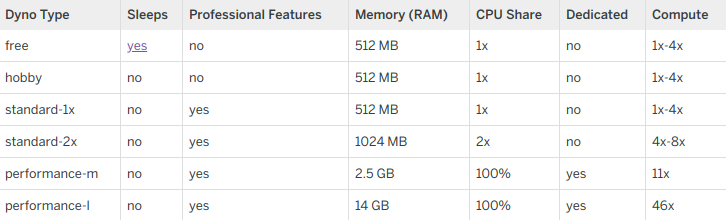
\includegraphics[scale=0.5]{dyno-type-features.png}  
	\caption[Tabel perbedaan fitur pada tipe dyno yang berbeda]{Tabel perbedaan fitur pada tipe dyno yang berbeda} 
	\label{fig:dyno-type-features} 
\end{figure}

Heroku menyediakan beberapa tipe dyno yang berbeda. Tiap tipe dyno memiliki sifat yang unik dan kinerja yang berbeda. Untuk semua pengguna Heroku, tersedia pilihan dyno tipe Free, Hobby, Standard, dan Performance. Perbedaan fitur untuk tiap tipe terdapat pada Gambar~\ref{fig:dyno-type-features}. Ada satu tipe dyno lagi, yaitu tipe Private. Dyno tipe Private hanya tersedia di Heroku Enterpise yang diperuntukkan untuk organisasi.

Fitur-fitur utama dyno adalah :
\begin{itemize}
\item \textit{Scalability}

Dyno dapat di-\textit{scale} secara horizontal dan vertikal. Untuk melakukan \textit{scale} secara horizontal (\textit{scale out}), tambahkan lebih banyak dyno. Contoh : menambah web dyno agar dapat menangani arus yang lebih besar. Untuk melakukan \textit{scale} secara vertikal (\textit{scale up}), gunakan dyno yang lebih besar. Dyno yang lebih besar berarti jumlah pemakaian memori RAM yang lebih besar. Jumlah RAM maksimal yang tersedia untuk aplikasi tergantung dari tipe dyno yang digunakan. \textit{Scale} secara horizontal dan vertikal ini adalah fitur yang tersedia untuk dyno tipe Standard dan Performance saja.

\item \textit{Redundancy}

Aplikasi dengan banyak dyno yang berjalan akan memiliki resiko kegagalan yang lebih rendah daripada yang sedikit. Jika ada dyno yang hilang, aplikasi dapat terus memproses permintaan sementara dyno yang hilang diganti. Dyno yang hilang biasanya langsung dimulai ulang, tapi terkadang membutuhkan waktu yang lama.

\item \textit{Isolation and security}

Semua dyno terisolasi dari dyno lain untuk alasan keamanan. Walaupun dyno tipe Free, Hobby, dan Standard terisolasi, dyno mungkin berbagi komputasi dasar yang sama. Heroku memiliki teknik tersendiri untuk memastikan penggunaannya adil. Di sisi lain, dyno tipe Performance dan Private tidak berbagi komputasi dasar yang sama dengan dyno lain. Hal ini membuat dyno tipe Performance dan Private memiliki kinerja yang lebih stabil dibanding dengan dyno tipe Free, Hobby, dan Standard. Selain memiliki sumber daya komputasi yang dikhususkan untuknya, dyno tipe Private juga memiliki jaringan virtual yang terisolasi.

\item \textit{Ephemeral filesystem}

Tiap dyno memiliki \textit{ephemeral filesystem}, dengan salinan kode dari hasil deploy terbaru. Saat masa hidup dyno, proses yang dijalankannya dapat menggunakan \textit{filesystem} ini sebagai tempat menulis sementara. Namun, dokumen yang ditulis tidak dapat dilihat oleh proses dari dyno lain dan dokumen yang ditulis akan dihapus saat dyno berhenti bekerja atau dimulai ulang.

\end{itemize}

\subsubsection{Dyno manager}
Dyno manager adalah bagian dari Heroku yang bertanggungjawab untuk menjaga dyno tetap berjalan. Dyno manager melakukan pekerjaan seperti memastikan dyno didaur ulang setidaknya satu kali sehari atau setiap dyno manager mendeteksi kesalahan di dalam aplikasi yang berjalan. Daur ulang dyno ini berlangsung secara transparan dan otomatis secara teratur dan tercatat.

Aplikasi yang menggunakan dyno tipe Free akan masuk mode \texttt{sleep} (tidur) jika tidak ada arus HTTP selama jangka waktu 30 menit. Ketika aplikasi yang tidur menerima arus HTTP, maka aplikasi tersebut akan terbangun. Hal ini menyebabkan aplikasi lebih lambat beberapa detik dari aplikasi yang menggunakan dyno tipe lain. Dyno tipe lain tidak memiliki mode sleep, dan akan selalu terjaga.

\subsubsection{Config vars}
Konfigurasi aplikasi dapat berubah-ubah tergantung lingkungannya. Misalnya, konfigurasi aplikasi saat pengembangan dapat berbeda saat aplikasi siap dirilis ke pengguna. Konfigurasi aplikasi dapat berupa informasi \textit{database}, informasi kredensial, atau informasi lain yang bersifat spesifik pada aplikasi. Konfigurasi ini harus diletakkan pada \textit{environment variable}, bukan di \textit{source code}. Dengan menggunakan \textit{environment variable}, konfigurasi dapat diubah secara terpisah. Selain itu, konfigurasi yang bersifat kredensial dapat terhindar dari tersimpan pada \textit{version control} (pengontrol versi, contoh : Git).

Heroku memungkinkan \textit{developer} untuk menjalankan aplikasi dengan konfigurasi yang dapat diubah dengan mudah. Konfigurasi tersebut diletakkan di luar dari \textit{source code} aplikasi. Konfigurasi dapat diubah secara independen tanpa harus mengubah \textit{source code}. Konfigurasi tersebut disimpan di dalam config vars.

Untuk mengatur config vars ada tiga cara : 
\begin{itemize}
\item Menggunakan Heroku CLI

Config var diatur menggunakan \textit{command shell}. Berikut perintah-perintah untuk mengatur config var menggunakan Heroku CLI:
\begin{itemize}
\item Menampilkan seluruh config var beserta nilainya : 

\begin{lstlisting}

	$ heroku config

\end{lstlisting}

\item Menampilkan nilai dari config var tertentu 
\begin{lstlisting}

	$ heroku config : get <config var>

\end{lstlisting}
Keterangan :
\begin{itemize}
\item \texttt{config var} : nama config var
\end{itemize}

\item Menambah config var

\begin{lstlisting}

	$ heroku config : set <config var> = <config value>

\end{lstlisting}
Keterangan :
\begin{itemize}
\item \texttt{config var} : nama config var
\item \texttt{config value} : nilai dari config var tersebut
\end{itemize}

\item Menghapus config var

\begin{lstlisting}

	$ heroku config : unset <config var>

\end{lstlisting}
Keterangan :
\begin{itemize}
\item \texttt{config var} : nama config var
\end{itemize}

\end{itemize}

\item Menggunakan Heroku Dashboard

\begin{figure}[H]
	\centering  
	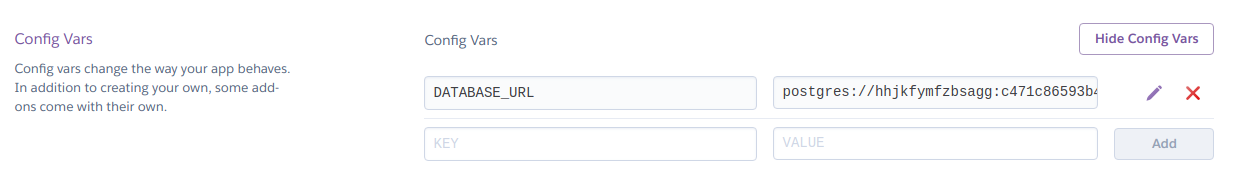
\includegraphics[width=\textwidth]{bluetape-config-vars-example.png}  
	\caption[Config vars pada dashboard Heroku]{Config vars pada dashboard Heroku} 
	\label{fig:bluetape-config-vars-example} 
\end{figure}

Config var dapat dilihat, ditambah, dan dihapus melalui menu \texttt{Settings} bagian config vars (Gambar~\ref{fig:bluetape-config-vars-example}).

\item Menggunakan Heroku Platform API

Config var dapat diatur dengan Heroku Platform API menggunakan HTTPS REST client sederhana dan data struktur data JSON. \textit{Developer} perlu Heroku \textit{access token} yang valid yang mewakili pengguna dengan izin yang tepat untuk aplikasi.

\end{itemize}

Config vars akan diperlakukan sebagai \textit{environment variable} oleh program. Contoh : \textit{environment variable} dapat diakses dengan getEnv() pada program dengan bahasa PHP.
 
Dalam mengatur config var, ada beberapa hal yang harus diperhatikan :
\begin{itemize}
\item Setiap config var ditambah atau dihapus, aplikasi akan dimulai ulang dan release baru akan dibuat.
\item Jika aplikasi menggunakan add-on, biasanya add-on tersebut akan menambahkan satu atau lebih config var ke aplikasi. Nilai dari config var tersebut mungkin diperbarui oleh penyedia add-on kapan saja.
\item Config var data (kombinasi dari semua kunci dan nilainya) tidak dapat melebihi 32kb per aplikasi
\item Nama config var tidak boleh diawali dengan garis bawah dua kali (\texttt{\_\_}).
\item Nama config var tidak bisa diawali dengan \texttt{HEROKU\_}, kecuali ditambahkan oleh platform Heroku sendiri.
\end{itemize}

\subsubsection{Add-ons}
Aplikasi biasanya memanfaatkan add-ons untuk menyediakan layanan penyokong seperti basis data, sistem antrean, layanan email, dan lainnya. Add-ons disediakan oleh Heroku atau pihak ketiga. \textit{Developer} dapat mencari add-ons di Elements Marketplace (\url{https://elements.heroku.com/addons}). 

Menambah add-ons selain add-ons Heroku Postgres dan Heroku Connect membutuhkan verifikasi akun. \textit{Developer} dapat menambah add-ons melalui tombol Install di Elements Marketplace atau dengan mengetikkan perintah berikut pada \textit{command shell} :
\begin{lstlisting}

	$ heroku addons:create <nama addons>:<tipe addons>

\end{lstlisting}
Keterangan :
\begin{itemize}
\item \texttt{<nama addons>} : nama addons
\item \texttt{<tipe addons>} : tipe addons
\end{itemize}

Contoh :
\begin{lstlisting}

	$ heroku addons:create heroku-redis:hobby-dev

\end{lstlisting}

\subsubsection{Slug}
Ketika platform Heroku menerima \textit{source code} aplikasi, heroku akan memulai proses \textit{build} berdasarkan \textit{source code}. Mekanisme \textit{build} biasanya tergantung pada bahasa pemrograman yang dipakai, tapi mengikuti pola yang sama. Mekanisme \textit{build} biasanya mengambil \textit{dependency} yang ditentukan, dan menciptakan aset yang diperlukan. \textit{Source code} untuk aplikasi, \textit{dependency}, dan hasil dari fase \textit{build} digabungkan ke dalam slug. 

Slug adalah gabungan dari \textit{source code}, \textit{dependency} yang diambil, \textit{language runtime}, dan hasil kompilasi atau keluaran yang dihasilkan oleh \textit{build system} yang siap untuk dieksekusi. Slug ini adalah aspek dasar dari eksekusi aplikasi. Slug berisi aplikasi yang sudah dikompilasi, digabungkan, dan siap untuk dijalankan.

Slug dikompilasi oleh slug compiler menggunakan buildpack. Buildpack akan mengambil aplikasi, \textit{dependency}, dan \textit{language runtime} dan kemudian menghasilkan slug. Buildpack bersifat \textit{open source}, sehingga memungkinkan \textit{developer} memperluas Heroku ke bahasa pemrograman lain dan \textit{framework}.

Apabila ada dokumen yang tidak diperlukan untuk menjalankan aplikasi, \textit{developer} dapat menambahkannya ke \texttt{.slugignore}. Dokumen ini harus dibuat di direktori \texttt{root}. Contoh dokumen yang mungkin ingin dimasukkan ke \texttt{.slugignore} :
\begin{itemize}
\item Dokumen pengolah gambar (contoh : dokumen .psd)
\item Dokumen desain (contoh : dokumen .pdf)
\item Data untuk pengujian
\end{itemize}

Contoh isi \texttt{.slugignore} :
\begin{lstlisting}
# Heres a comment
*.psd
*.pdf
/test
/spec
\end{lstlisting}

Ukuran slug dapat terlihat di akhir kompilasi (apabila kompilasi berhasil). Maksimum ukuran slug adalah 500 MB. Ukuran slug bervariasi berdasarkan bahasa atau \textit{framework} yang digunakan, banyak \textit{dependency} yang ditambahkan, dan faktor lain dari aplikasi. Slug yang ukurannya lebih kecil dapat ditransfer ke dyno manager dengan lebih cepat.

\subsubsection{Buildpack}
Buildpack bertanggung jawab untuk mengubah \textit{source code} menjadi slug, sehingga dyno dapat mengeksekusinya. Buildpack terdiri dari sekumpulan \textit{script} yang ditulis dalam bahasa pemrograman yang sama dengan \textit{source code}. Script tersebut akan mengambil \textit{dependency}, mengeluarkan aset atau kode yang sudah dikompilasi, dan sebagainya. Keluaran ini akan digabungkan ke dalam slug oleh slug compiler.

Heroku memiliki sekumpulan \textit{officially supported buildpack} yang tersedia secara default untuk semua aplikasi Heroku selama kompilasi slug. Daftar \textit{officially supported buildpack} terdapat pada Gambar~\ref{fig:heroku-buildpack-table}. Kolom \texttt{Buildpack} menyatakan nama buildpack dan kolom \texttt{shorthand} menyatakan nama panggil buildpack saat di CLI.

\begin{figure}[H]
	\centering  
	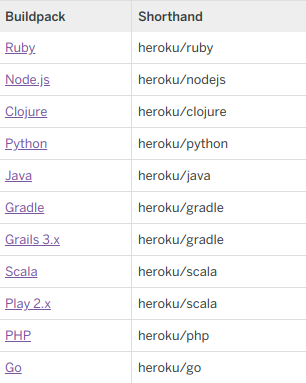
\includegraphics[scale=0.5]{heroku-buildpack-table.png}  
	\caption[Tabel buildpack heroku]{Tabel buildpack heroku} 
	\label{fig:heroku-buildpack-table} 
\end{figure}

Heroku akan mencari buildpack yang sesuai dan menggunakannya untuk mengompilasi aplikasi. Jika build sukses, buildpack yang sudah terdeteksi sesuai akan secara permanen diatur untuk push selanjutnya. Buildpack yang telah dimodifikasi dapat dipakai untuk mendukung bahasa atau framework yang tidak dapat di cakup oleh buildpack resmi.

Biasanya buildpack yang dipakai oleh aplikasi hanya satu, tapi ada beberapa kasus buildpack yang dipakai tidak cukup hanya satu. Beberapa kasus tersebut adalah :
\begin{itemize}
\item Menjalankan buildpack untuk tiap bahasa pemrograman yang aplikasi gunakan. Contohnya, menjalankan JavaScript buildpack untuk aset dan buildpack Ruby untuk aplikasi.
\item Menjalankan proses daemon seperti \texttt{pgbouncer} dengan aplikasi.
\item Menarik \textit{dependency} sistem dengan apt.
\end{itemize}

Berikut adalah perintah-perintah dasar buildpack yang dapat diketikkan pada \textit{command shell} :
\begin{itemize}
\item Mengatur buildpack yang dipakai saat aplikasi pertama kali dibuat
\begin{lstlisting}

	$ heroku create myapp --buildpack <nama buildpack>
	
\end{lstlisting}
Keterangan :
\begin{itemize}
\item \texttt{<nama buildpack>} : nama panggil buildpack yang ingin dipakai, contoh : \texttt{heroku/php}.
\end{itemize}

Buildpack juga dapat secara eksplisit diatur di dalam app.json sehingga aplikasi yang dibuat menggunakan tombol Heroku dapat menggunakan buildpack yang telah dimodifikasi.

\item Mengubah dengan mengatur nilai buildpack

\begin{lstlisting}

	$ heroku buildpacks:set <nama buildpack>
	
\end{lstlisting}
Keterangan :
\begin{itemize}
\item \texttt{<nama buildpack>} : nama panggil buildpack yang ingin dipakai, contoh : \texttt{heroku/php}.
\end{itemize}

\item Menghilangkan buildpack dari aplikasi

\begin{lstlisting}

	$ heroku buildpacks:remove <nama buildpack>
	
\end{lstlisting}
Keterangan :
\begin{itemize}
\item \texttt{<nama buildpack>} : nama panggil buildpack yang ingin dipakai, contoh : \texttt{heroku/php}.
\end{itemize}

\item Mencari buildpack

\begin{lstlisting}

	$ heroku buildpacks:search <kata kunci>
	
\end{lstlisting}
Keterangan :
\begin{itemize}
\item \texttt{<kata kunci>} : kata kunci pencarian, misalnya : bahasa pemrograman yang dipakai. Contoh : \texttt{elixir}.
\end{itemize}

\item Menampilkan informasi buildpack

\begin{lstlisting}

	$ heroku buildpacks:info <nama buildpack>
	
\end{lstlisting}
Keterangan :
\begin{itemize}
\item \texttt{<nama buildpack>} : nama panggil buildpack yang ingin dipakai, contoh : \texttt{heroku/php}.
\end{itemize}

\item Mengembalikan aplikasi ke buildpack awalnya

\begin{lstlisting}

	$ heroku buildpacks:clear
	
\end{lstlisting}

\item Mengatur urutan eksekusi buildpack

\begin{lstlisting}

	$ heroku buildpacks:set --index <index> <nama buildpack>

\end{lstlisting}
Keterangan :
\begin{itemize}
\item \texttt{<index>} : urutan eksekusi buildpack
\item \texttt{<nama buildpack>} : nama panggil buildpack yang ingin dipakai, contoh : \texttt{heroku/php}.
\end{itemize}

\item Melihat daftar buildpack

\begin{lstlisting}

	$ heroku buildpacks

\end{lstlisting}

\end{itemize}

\subsubsection{Stack}
Stack adalah sistem operasi yang dikelola dan dipelihara oleh Heroku. Stack biasanya berlandaskan distribusi dari Linux yang ada, seperti Ubuntu. \textit{Developer} dapat menentukan stack yang dipakai, dan buildpack akan mengubah \textit{source code} menjadi paket yang dapat dieksekusi dengan stack tersebut. Saat skripsi ini dibuat, Heroku menyediakan tiga stack : Cedar-14, Heroku-16, dan Heroku-18. Cedar-14 berbasis Ubuntu 14.04 dan didukung sampai bulan April tahun 2019. Heroku-16 berbasis Ubuntu 16.04 dan didukung sampai bulan April tahun 2021. Heroku-18 berbasis Ubuntu 18.04 dan didukung sampai bulan April tahun 2023. Semua buildpack dari Heroku dapat bekerja dengan ketiga stack tersebut, namun buildpack yang merupakan hasil modifikasi belum tentu dapat bekerja dengan semua stack.

Untuk melihat stack yang dipakai oleh aplikasi, \textit{developer} dapat mengetikkan perintah berikut pada \textit{command shell}:
\begin{lstlisting}

	$ heroku stack

\end{lstlisting}

Untuk mengganti stack yang dipakai, \textit{developer} dapat mengetikkan perintah berikut pada \textit{command shell}:
\begin{lstlisting}

	$ heroku stack:set <stack>

\end{lstlisting}
Keterangan :
\begin{itemize}
\item \texttt{<stack>} dapat diisi dengan \texttt{cedar-14}, \texttt{heroku-16}, atau \texttt{heroku-18}.
\end{itemize}

\subsubsection{Region}
Aplikasi di dalam Heroku dapat disebarkan ke lokasi geografis yang berbeda. Lokasi yang tersedia untuk suatu aplikasi tergantung pada Runtime yang dipakai oleh aplikasi (Common Runtime atau Private Space). Untuk aplikasi yang memakai Common Runtime, \textit{developer} perlu menyebutkan region aplikasi saat membuat aplikasi. Untuk aplikasi yang memakai Private Space, region diatur saat membuat Private Space. Apabila \textit{developer} tidak menyebutkan region yang dipakai, maka region akan diisi secara otomatis sebagai \texttt{us} (apabila memakai Common Runtime) atau \texttt{virginia} (apabila memakai Private Spaces).

Region berpengaruh terhadap add-ons. Apabila add-ons tidak tersedia di region yang sama dengan aplikasi, maka add-ons akan gagal terpasang. Region juga dapat mempengaruhi cara kerja SSL.

Berikut perintah-perintah dasar region yang dapat diketikkan pada \textit{command shell} :
\begin{itemize}
\item Memeriksa region yang tersedia di Heroku

\begin{lstlisting}

	$ heroku regions

\end{lstlisting}

\item Mengatur region aplikasi

\begin{lstlisting}

	$ heroku create --region <id region>

\end{lstlisting}
Keterangan :
\begin{itemize}
\item \texttt{<id region>} : id region yang ingin dipakai, contoh : \texttt{eu}.Id region bisa dilihat dengan memeriksa daftar region yang tersedia.
\end{itemize}

\item Memeriksa region yang dipakai oleh aplikasi

\begin{lstlisting}

	$ heroku info

\end{lstlisting}

\end{itemize}

\subsubsection{Releases}
Setiap ada deploy baru, perubahan di config vars, dan perubahan di daftar add-ons, Heroku akan membuat release baru dan memulai ulang aplikasi. Releases adalah buku besar yang mencatat setiap release tersebut. \textit{Developer} dapat melihat catatan releases ini dengan menggunakan perintah :
\begin{lstlisting}

	$ heroku releases

\end{lstlisting}

Isi dari releases adalah satu atau lebih baris dari release yang tiap barisnya memiliki format : 
\begin{lstlisting}

	<versi deploy> Deploy <commit hash> <username \textit{developer}> <waktu deploy> 

\end{lstlisting}

Contoh isi releases :
\begin{lstlisting}

	== demoapp Releases
	v103 Deploy 582fc95  jon@heroku.com   2013/01/31 12:15:35
	v102 Deploy 990d916  jon@heroku.com   2013/01/31 12:01:12
	
\end{lstlisting}

Releases ini berguna saat \textit{developer} ingin mengembalikan aplikasi ke deploy lama. Cara mengembalikan aplikasi ke deploy lama dengan mengetikkan perintah berikut pada \textit{command shell}:
\begin{lstlisting}

	$ heroku releases:rollback <version>

\end{lstlisting}
Keterangan :
\begin{itemize}
\item \texttt{<version>} : versi deploy
\end{itemize}

Contoh :
\begin{lstlisting}

	$ heroku releases:rollback v102

\end{lstlisting}

\subsubsection{Log}
Log adalah catatan setiap proses yang terjadi di aplikasi. Heroku menggunakan Logplex untuk menyampaikan log ini. Logplex akan secara otomatis menambahkan entri log baru dari semua dyno yang berjalan di aplikasi, dan juga komponen lain seperti router. \textit{Developer} dapat memeriksa log dengan cara mengetikkan perintah berikut pada \textit{command shell}:
\begin{lstlisting}

	$ heroku logs

\end{lstlisting}

Contoh isi log adalah :
\begin{lstlisting}

	2013-02-11T15:19:10+00:00 heroku[router]: at=info method=GET path=/articles/custom-domains host=mydemoapp.heroku.com fwd=74.58.173.188 dyno=web.1 queue=0 wait=0ms connect=0ms service=1452ms status=200 bytes=5783
	2013-02-11T15:19:10+00:00 app[web.2]: Started GET "/" for 1.169.38.175 at 2013-02-11 15:19:10 +0000
	2013-02-11T15:19:10+00:00 app[web.1]: Started GET "/" for 2.161.132.15 at 2013-02-11 15:20:10 +0000

\end{lstlisting}

\subsection{Deploy Perangkat Lunak}
Heroku menggunakan Git sebagai sarana  utama untuk melakukan deploy aplikasi. Deploy adalah proses penyebaran aplikasi dari satu lingkungan ke lingkungan lain, misalnya dari lingkungan mesin \textit{developer} aplikasi ke lingkungan heroku. Namun, Heroku juga menyediakan cara lain untuk melakukan deploy :
\begin{itemize}
\item Docker
\item GitHub
\item Tombol \texttt{Deploy} di dashboard Heroku
\item WAR deployment
\end{itemize}

\subsubsection{Deploy Menggunakan Git}
Untuk melakukan deploy menggunakan Git, \textit{developer} harus sudah memasang Git. \textit{Developer} dapat mengikuti petunjuk unduhan pada \url{https://git-scm.com}. Sebelum \textit{developer} dapat melakukan deploy dengan Git, \textit{developer} perlu menginisialisasi git. Berikut perintah-perintah yang harus dijalankan pada \textit{command shell} :
\begin{lstlisting}

	$ git init
	$ git add .
	$ git commit -m "<message>"

\end{lstlisting}
Keterangan :
\begin{itemize}
\item \texttt{<message>} : pesan yang mewakili commit.
\end{itemize}

Setelahnya, \textit{developer} dapat membuat aplikasi Heroku. Setiap aplikasi Heroku dibuat, maka \texttt{git remote} secara otomatis juga dibuat. \textit{Developer} dapat memeriksanya dengan mengetikkan perintah berikut pada \textit{command shell} :
\begin{lstlisting}

	$ git remote // Untuk daftar nama remote saja
	$ git remote -v // Untuk informasi yang lebih detail

\end{lstlisting}

Untuk mengubah nama remote, \textit{developer} dapat mengetikkan perintah berikut pada \textit{command shell} :
\begin{lstlisting}

	$ git remote rename <nama lama> <nama baru>

\end{lstlisting}
Keterangan :
\begin{itemize}
\item \texttt{<nama lama>} : nama remote yang ingin diganti.
\item \texttt{<nama baru>} : nama baru untuk remote tersebut.
\end{itemize}

Untuk melakukan deploy, \textit{developer} dapat mengetikkan perintah berikut pada \textit{command shell} :
\begin{lstlisting}

	$ git push <nama remote> <nama branch>

\end{lstlisting}
Keterangan :
\begin{itemize}
\item \texttt{<nama remote>} : nama remote dari tujuan deploy. Bila \textit{developer} tidak mengubah nama remote, nama remotenya adalah \texttt{heroku}. 
\item \texttt{<nama branch>} : nama cabang dari tujuan deploy. Heroku secara otomatis membuat satu cabang bernama \texttt{master}.
\end{itemize}

\subsubsection{Deploy Menggunakan Docker}
Untuk melakukan deploy menggunakan Docker, \textit{developer} harus sudah memasang Docker dan telah masuk ke akun Heroku (\texttt{heroku login}). Setelah itu, \textit{developer} harus mengikuti langkah-langkah ini :
\begin{itemize}
\item Masuk ke Container Registry
\begin{lstlisting}

	$ heroku container:login

\end{lstlisting}

\item Clone source code contoh dari Alpine
\begin{lstlisting}

	$ git clone https://github.com/heroku/alpinehelloworld.git

\end{lstlisting}

\item Membuat aplikasi Heroku baru
\begin{lstlisting}

	$ heroku create

\end{lstlisting}

\item Membangun image dan melakukan deploy ke Container Registry
\begin{lstlisting}

	$ heroku container:push web

\end{lstlisting}

\item Melepaskan image ke aplikasi
\begin{lstlisting}

	$ heroku container:release web

\end{lstlisting}
\item Membuka aplikasi
\begin{lstlisting}

	$ heroku open

\end{lstlisting}
\end{itemize}

\subsubsection{Deploy Menggunakan GitHub}
\begin{figure}[H]
	\centering  
	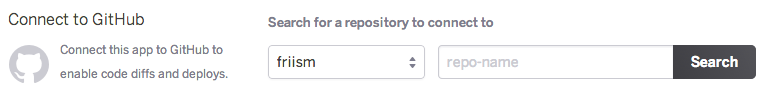
\includegraphics[scale=0.5]{deploy-github-dashboard.jpg}  
	\caption[Deploy menggunakan Github Dashboard]{Deploy menggunakan Github Dashboard} 
	\label{fig:deploy-github-dashboard} 
\end{figure}
Deploy dengan cara ini membuat Heroku dapat dengan otomatis melakukan deploy ke GitHub apabila build berhasil. \textit{Developer} perlu mengaktifkan GitHub integration terlebih dahulu sebelum dapat melakukan deploy. Setelah itu, \textit{developer} harus melakukan autentikasi dengan akun GitHub. Autentikasi ini hanya perlu dilakukan satu kali per satu akun Heroku. Setelah itu, \textit{developer} dapat memilih repository yang ingin disambungkan dengan aplikasi Heroku (Gambar~\ref{fig:deploy-github-dashboard}).

\begin{figure}[H]
	\centering  
	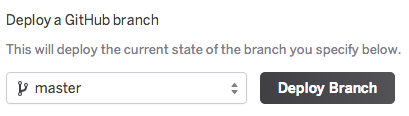
\includegraphics[scale=0.5]{deploy-github-manual.jpg}  
	\caption[Deploy menggunakan Github secara manual]{Deploy menggunakan Github secara manual} 
	\label{fig:deploy-github-manual} 
\end{figure}
\begin{figure}[H]
	\centering  
	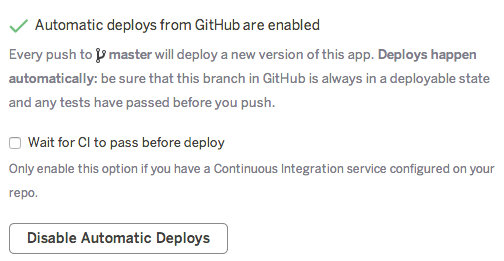
\includegraphics[scale=0.5]{deploy-github-automatic.jpg}  
	\caption[Deploy menggunakan Github secara otomatis]{Deploy menggunakan Github secara otomatis} 
	\label{fig:deploy-github-automatic} 
\end{figure}
Ada dua cara untuk melakukan deploy, yaitu secara manual dan secara otomatis. Untuk cara manual, \textit{developer} melakukan deploy dari GitHub (Gambar~\ref{fig:deploy-github-manual}). Untuk cara otomatis, \textit{developer} harus mengaktifkan "Automatic deploys from GitHub" (Gambar~\ref{fig:deploy-github-automatic}).

\subsubsection{Deploy Langsung di situs Heroku}
Tombol "Deploy to Heroku" memungkinkan pengguna untuk melakukan deploy aplikasi tanpa meninggalkan situs Heroku dan hampir tidak memerlukan konfigurasi. Penggunaan tombol ini ideal untuk pelanggan, dan pemelihara proyek yang bersifat open-source. Sebelum dapat melakukan deploy dengan cara ini, aplikasi harus memiliki dokumen \texttt{app.json} yang sah di direktori root, dan source code aplikasi harus berada di repository GitHub.

\texttt{app.json} adalah dokumen berisi deskripsi aplikasi web. Isinya dapat berupa environment variable, add-ons, dan informasi lain yang diperlukan untuk menjalankan aplikasi pada Heroku. Heroku tidak mewajibkan \textit{developer} menuliskan informasi tertentu, tapi Heroku merekomendasikan untuk setidaknya menuliskan nama aplikasi(\texttt{name}), deskripsi aplikasi (\texttt{description}), dan logo aplikasi (\texttt{logo}). Berikut contoh isi dari \texttt{app.json} :
\begin{lstlisting}

{
  "name": "Node.js Sample",
  "description": "A barebones Node.js app using Express 4",
  "repository": "https://github.com/heroku/node-js-sample",
  "logo": "https://node-js-sample.herokuapp.com/node.png",
  "keywords": ["node", "express", "static"]
}

\end{lstlisting}

\subsubsection{WAR Deployment}
WAR (Web Application ARchive) adalah jenis dokumen arsip yang digunakan untuk membungkus aplikasi web. Dokumen ini dapat berisi halaman web statis, dokumen XML, dan lain-lain. \cite{etzkorn2017introduction}
 
Heroku mendukung deploy dokumen WAR melalui Git deployment dan melalui Heroku Maven plugin. Setelan standar server untuk keduanya adalah Tomcat 8.

\subsection{Basis Data dan Manajemen Data}
Heroku menyediakan tiga layanan data untuk semua pelanggan :
\begin{itemize}
\item Heroku Postgres
\item Heroku Redis
\item Apache Kafka
\end{itemize}
Heroku juga menyediakan pilihan lain untuk pelanggan Heroku Enterprise, yaitu Heroku Connect. Selain itu, Heroku juga memungkinkan penggunaan layanan data dari pihak ketiga. Layanan data dari pihak ketiga ini tersedia sebagai add-ons.

\subsubsection{Heroku Postgres}
Heroku Postgres adalah basis data SQL yang disediakan secara langsung oleh Heroku. Heroku Postgres dapat diakses oleh bahasa apapun dengan PostgreSQL driver. Heroku secara otomatis menambahkan add-ons Heroku Postgres setiap aplikasi dibuat, sehingga \textit{developer} tidak perlu menambahkannya secara manual. Namun, \textit{developer} dapat menambahkannya secara manual, dengan mengetikkan perintah berikut pada \textit{command shell} :
\begin{lstlisting}
	
	$ heroku addons:create heroku-postgresql:<PLAN_NAME>
	
\end{lstlisting}
Keterangan :
\begin{itemize}
\item \texttt{<PLAN\_NAME>} : nama plan Heroku Postgres yang ingin dipakai. Heroku secara otomatis menggunakan Heroku Postgres tipe \texttt{hobby-dev}.
\end{itemize}

Heroku Postgres memiliki lima plan :
\begin{itemize}
\item Hobby Tier : untuk aplikasi dengan toleransi gagal bekerja sampai 4 jam per bulan.
\item Standard Tier : untuk aplikasi dengan toleransi gagal bekerja sampai 1 jam per bulan.
\item Premium Tier : untuk aplikasi dengan toleransi gagal bekerja sampai 15 menit per bulan.
\item Private Tier : untuk pengguna Heroku Enterprise, memiliki toleransi gagal bekerja sampai 15 menit per bulan.
\item Shield Tier : untuk pengguna Heroku Enterprise yang menginginkan basis data yang compliance-capable, memiliki toleransi gagal bekerja sampai 15 menit per bulan.
\end{itemize}

Gambar~\ref{fig:heroku-postgres-plan-table} menunjukkan tabel perbedaan antara plan. Hanya plan Hobby yang gratis. Plan lain memiliki harga yang bervariasi berdasarkan ukuran RAM, batas penyimpanan, dan batas koneksi yang bisa dibuat.
\begin{figure}[H]
	\centering  
	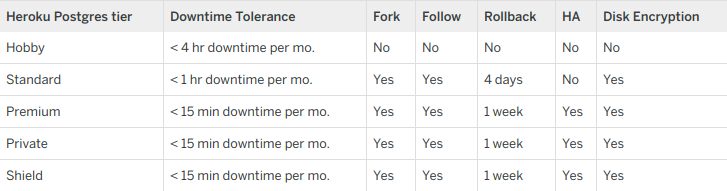
\includegraphics[scale=0.5]{heroku-postgres-plan-table.png}  
	\caption[Tabel plan Heroku Postgres]{Tabel plan Heroku Postgres} 
	\label{fig:heroku-postgres-plan-table} 
\end{figure}

Semua plan memiliki fitur yang sama :
\begin{itemize}
\item Dapat mengelola layanan basis data secara menyeluruh dengan fitur \textit{automatic health checks}
\item Write-ahead log (WAL) menjauh dari tempat penyimpanan setiap 60 detik, memastikan resiko kehilangan data dan kesalahan lainnya seminimal mungkin
\item Backup basis data harian menggunakan PG Backups (opsional, tapi gratis)
\item Dataclips untuk berbagi data dan query yang mudah dan aman
\item Akses psql/libpq dengan SSL-protected
\item Menjalankan Postgres 9.4, 9.5, 9.6, atau 10 tanpa modifikasi
\item Ekstensi Postgres
\item Fitur web UI (\url{https://data.heroku.com/})
\end{itemize}

\textit{Developer} juga dapat menambahkan versi yang ingin dipakai dengan cara menambahkan \texttt{--version} di belakang perintah tersebut, contoh :
\begin{lstlisting}
	
	$ heroku addons:create heroku-postgresql:<PLAN_NAME--version=9.5
	
\end{lstlisting}
Secara otomatis, Heroku menggunakan versi paling baru dari Heroku Postgres. Saat skripsi ini ditulis, versi terbaru adalah versi 10.

Setelah dipasang, Heroku akan secara otomatis menambahkan config var \texttt{DATABASE\_URL} ke aplikasi. Apabila Heroku Postgres yang dipakai ada lebih dari satu, nama config var akan menjadi \texttt{HEROKU\_POSTGRESQL\_<COLOR>\_URL} dengan <COLOR> adalah nama warna yang dihasilkan secara acak. Contoh : \texttt{HEROKU\_POSTGRESQL\_<BLUE>\_URL}.

Apabila \textit{developer} menggunakan lebih dari satu basis data, \textit{developer} dapat mengatur basis data utama. Basis data utama dapat diatur dengan mengetikkan perintah berikut pada \textit{command shell} :
\begin{lstlisting}
	
	$ heroku pg:promote <database_url>
	
\end{lstlisting}
Keterangan :
\begin{itemize}
\item \texttt{<database\_url>} : url dari basis data.
\end{itemize}

Apabila \textit{developer} ingin berbagi Heroku Postgres kepada banyak aplikasi, \textit{developer} dapat mengetikkan perintah berikut pada \textit{command shell} : 
\begin{lstlisting}

	$ heroku addons:attach <originating_app>::DATABASE --app <receiver-app>
	
\end{lstlisting}
Keterangan :
\begin{itemize}
\item \texttt{<originating\_app>} : nama aplikasi yang memiliki basis data yang ingin dibagi ke aplikasi lain. 
\item \texttt{<receiver-app>} : nama aplikasi yang akan menerima basis data dari aplikasi lain.
\end{itemize}

\textit{Developer} dapat berhenti berbagi basis data dengan mengetikkan perintah berikut pada \textit{command shell} :
\begin{lstlisting}

	$ heroku addons:detach <database_url> --app <application_name>

\end{lstlisting}
Keterangan :
\begin{itemize}
\item \texttt{<database\_url>} : url dari basis data
\item \texttt{<application\_name>} : nama aplikasinya.
\end{itemize}

Berikut adalah perintah-perintah dasar dari Heroku Postgres yang dapat diketikkan pada \textit{command shell}:
\begin{itemize}
\item Melihat semua basis data milik aplikasi dan karakteristiknya

\begin{lstlisting}

	$ heroku pg:info

\end{lstlisting}

\item Mengawasi status basis data secara terus menerus

\begin{lstlisting}

	$ watch heroku pg:info

\end{lstlisting}

\item Mengadakan sesi \texttt{psql} dengan basis data

\begin{lstlisting}

	$ heroku pg:psql

\end{lstlisting}
atau
\begin{lstlisting}

	$ heroku pg:psql <database_name>

\end{lstlisting}
Keterangan :
\begin{itemize}
\item \texttt{<database\_name>} diisi dengan nama basis data atau cukup warna basis data (misal : \texttt{gray}).
\end{itemize}

\item Menarik data dari basis data Heroku Postgres ke basis data di mesin lokal

\begin{lstlisting}

	$ heroku pg:pull

\end{lstlisting}

\item Memasukkan data dari basis data di mesin lokal ke basis data di Heroku Postgres

\begin{lstlisting}

	$ heroku pg:push <nama_db_lokal> <nama_db_heroku> --app <nama_aplikasi>

\end{lstlisting}

\item Melihat daftar query yang berjalan

\begin{lstlisting}

	$ heroku pg:ps
	// Contoh hasil :
	procpid |         source            |   running_for   | waiting |         query
	---------+---------------------------+-----------------+---------+-----------------------
	   31776 | psql                      | 00:19:08.017088 | f       | <IDLE> in transaction
	   31912 | psql                      | 00:18:56.12178  | t       | select * from hello;
	   32670 | Heroku Postgres Data Clip | 00:00:25.625609 | f       | BEGIN READ ONLY; select 'hi'
	(3 rows)
	
\end{lstlisting}

\item Menghentikan query yang berjalan

\begin{lstlisting}

	$ heroku pg:kill <procpid>

\end{lstlisting}

\item Menghentikan query yang berjalan secara paksa

\begin{lstlisting}

	$ heroku pg:kill --force <procpid>

\end{lstlisting}

\item Menghentikan semua query yang berjalan

\begin{lstlisting}

	$ heroku pg:killall

\end{lstlisting}

\item Menghapus semua data di dalam basis data

\begin{lstlisting}

	$ heroku pg:reset <nama database>

\end{lstlisting}
\end{itemize}

Basis data Heroku Postgres dapat diakses secara langsung oleh komputer. Informasi yang dibutuhkan untuk mengakses data dari komputer dapat dilihat dengan mengetikkan perintah :
\begin{lstlisting}

	$ heroku pg:credentials DATABASE
	
\end{lstlisting}
atau
\begin{lstlisting}

	$ heroku config | grep HEROKU_POSTGRESQL
	
\end{lstlisting}
Pada saat akan melakukan koneksi langsung di komputer, \textit{developer} harus memastikan pengaturan \texttt{sslmode=require} pada pengaturan SSL.

\subsubsection{Heroku Redis}
Heroku Redis adalah basis data berbasis \textit{key-value store} yang bersifat \textit{in-memory}. Heroku dijalankan oleh Heroku dan dikelola sebagai add-on Heroku Redis dapat diakses oleh bahasa apapun dengan Redis driver. Cara memasang add-on Heroku Redis pada \textit{command shell}:
\begin{lstlisting}
	
	$ heroku addons:create heroku-redis: <PLAN_NAME>
	
\end{lstlisting}
Keterangan :
\begin{itemize}
\item \texttt{<PLAN\_NAME>} : tipe Heroku Redis yang ingin dipakai. Heroku Redis memiliki dua tipe : Hobby Dev dan Premium. Hobby Dev gratis, sedangkan Premium berbayar. Perbedaannya terletak pada jumlah memori dan batas koneksi yang dapat dibuat.
\end{itemize}

Heroku Redis memiliki kelebihan sebagai berikut :
\begin{itemize}
\item Memiliki analisa performa yang dapat membantu menemukan masalah basis data dengan mudah
\item Heroku dapat diskala sesuai kebutuhan memori dan koneksi.
\end{itemize}

\subsubsection{Apache Kafka}
Apache Kafka adalah salah satu add-on di Heroku yang disediakan oleh Kafka yang berintegrasi penuh dengan Heroku. Apache Kafka dideskripsikan Kafka dideskripsikan oleh Heroku sebagai add-on yang memungkinkan \textit{developer} mendistribusikan aplikasi yang dapat menangani jutaan event dan miliaran transaksi. Kafka didesain untuk memindahkan \textit{ephemeral data} yang sangat besar dengan reliabilitas yang tinggi dan toleran akan kerusakan.

\textit{Developer} harus memasang Python 2.7, node 8.x, .NET Framework, dan Visual C++ Build Tools terlebih dahulu sebelum memasang Apache Kafka. Setelah itu, \textit{developer} mengetikkan perintah :
\begin{lstlisting}
	
	$ heroku plugins:install heroku-kafka
	
\end{lstlisting}

\subsection{Verifikasi Akun}
Heroku membutuhkan identitas terpercaya dan kontak dari pengguna. Heroku menganggap mempunyai informasi kartu kredit adalah cara yang paling dapat diandalkan untuk mendapatkan informasi kontak yang terverifikasi. Verifikasi akun juga membantu Heroku untuk menghindari penyalahgunaan.

Verifikasi akun dibutuhkan untuk :
\begin{itemize}
\item Menggunakan lebih dari satu dyno di dalam aplikasi.
\item Menambah add-on, termasuk yang gratis. Pengecualian untuk Heroku Postgres dan Heroku Connect.
\item Mengubah domain aplikasi.
\item Menerima transfer dari aplikasi yang memiliki sumber daya berbayar.
\item Menambah batas standar penggunaan one-off dyno.
\item Memiliki lebih dari 5 aplikasi dalam satu waktu.  Akun yang terverifikasi dapat memiliki sampai 100 aplikasi.
\end{itemize}

Cara melakukan verifikasi akun Heroku :
\begin{itemize}
\item Pergi ke Account Settings (\url{https://dashboard.heroku.com/account})
\item Menekan tab Billing
\item Menekan tombol Add Credit Card
\end{itemize}

Kartu kredit yang diterima oleh Heroku adalah kartu Visa, MasterCard, American Express, Discover dan JCB. Kartu debit juga diterima untuk kartu Visa, MasterCard atau JCB. Kartu lain tidak diterima. Beberapa bank mungkin mensyaratkan penahanan satu dollar oleh pelaku verifikasi sebelum kartu dapat dikonfirmasi.

\section{Cron ~\cite{vixie1cron}}
\label{cron}
Cron adalah program yang menjalankan command (perintah) yang tertera di file crontab pada jadwal tertentu di latar belakang secara otomatis. File crontab dapat ditemukan di direktori /var/spool/cron/crontabs. Crontab di  direktori ini sebaiknya tidak diakses secara langsung, melainkan menggunakan command crontab. File crontab juga dapat ditemukan di direktori /etc atau subdirektori /etc. File crontab di direktori tersebut adalah file system crontab.

Setiap command di crontab diawali dengan lima penanda waktu dan diikuti dengan nama user (jika berada di file system crontab). Lima penanda waktu tersebut secara berurutan adalah :
\begin{itemize}
\item minute : menandakan tiap menit berapa command dijalankan. Value yang valid adalah angka 0-59 atau tanda asterisk (*).
\item hour : menandakan tiap jam berapa command dijalankan. Value yang valid adalah angka 0-23 atau tanda asterisk (*).
\item day of the month : menandakan tiap tanggal berapa command dijalankan. Value yang valid adalah angka 1-31 atau tanda asterisk (*).
\item month : menandakan tiap bulan berapa command dijalankan. Value yang valid adalah angka 1-12 atau tanda asterisk (*).
\item day of the week : menandakan tiap hari apa command dijalankan. Value yang valid adalah angka 0-7 atau tanda asterisk (*) atau "Sun". Hari minggu dapat ditulis dengan angka 0 atau 7 atau "Sun".
\end{itemize}

Contoh penulisan command di crontab :
\begin{lstlisting}
0 12 * * * /home/myscripts/lunch.sh
\end{lstlisting}
Pada contoh di atas, cron akan menjalanksan script lunch.sh pada direktori /home/myscripts setiap hari pada jam 12:00. Tanda asterisk menandakan eksekusi dilakukan dari range value terendah sampai value tertinggi.

Penanda waktu boleh memiliki value lebih dari satu. Penanda waktu yang memiliki value lebih dari satu ditulis dalam bentuk range, list, atau step. Range ditulis dalam format dua value yang dipisahkan dengan tanda hubung (-). Range bersifat inklusif. Contoh : 8-11 untuk hour berarti command akan dieksekusi pada jam 8, 9, 10, dan 11. List ditulis dalam format dua atau lebih value yang dipisahkan dengan koma. Contoh : 1,5,7. Range dan list dapat disatukan. Contoh : 1,2,8-12. Step ditulis dalam format : range / <number>. Contoh : '0-23/2' untuk hour. Tanda tersebut berarti eksekusi dijalankan setiap dua jam sekali. Tanda asterisk juga dapat digunakan untuk menggantikan range. Contoh : */4 untuk hour. Tanda tersebut berarti eksekusi dijalankan setiap empat jam sekali.

Nama juga dapat digunakan untuk penanda waktu month atau day of week. Cukup dengan menggunakan tiga huruf pertama dari kata bahasa Inggrisnya tanpa menghiraukan huruf besar atau huruf kecil. Namun, nama tidak bisa dipakai untuk range atau list.  

Selain itu, kelima penanda waktu dapat diganti dengan salah satu "nickname" berikut :
\begin{itemize}
\item @reboot : Eksekusi sekali saat startup.
\item @yearly : Eksekusi setiap tahun (setiap tanggal 1 Januari), "0 0 1 1 *"
\item @anually : Sama seperti @yearly.
\item @monthly : Eksekusi setiap bulan, "0 0 1 * *".
\item @weekly : Eksekusi setiap minggu, "0 0 * * 0".
\item @daily : Eksekusi setiap hari (jam 00:00), "0 0 * * *"
\item @midnight : Sama seperti @daily.
\item @hourly : Eksekusi setiap jam, "0 * * * *"
\end{itemize}

Baris kosong, spasi di awal baris, dan tab akan diabaikan oleh cron. Baris yang karakter bukan spasi pertamanya  adalah \# akan dianggap sebagai comment (komentar) dan akan diabaikan. Comment tidak boleh diletakkan di baris yang sama dengan command karena comment tersebut akan dianggap sebagai bagian dari command.

\section{Gmail API ~\cite{gmail-api}}
\label{sec:gmail-api}
Gmail adalah layanan email yang disediakan oleh Google LLC. Gmail API dapat digunakan untuk mengakses email Gmail.

\subsection{Resource}
Gmail API menyediakan beberapa jenis \textit{resource} :
\begin{itemize}
\item Message

Message merepresentasikan pesan dalam email. Message hanya bisa dibuat atau dihapus. Tidak ada properti dari message yang bisa diubah selain label yang diberikan ke message.

\item Label

Label berfungsi sebagai sarana utama untuk mengelompokkan dan mengatur message dan thread. Label mempunyai hubungan banyak ke banyak dengan message. Artinya, satu message dapat memiliki beberapa label dan satu label dapat diberikan ke beberapa message.

Label ada dua jenis : label sistem dan label pengguna. Contoh label sistem adalah label \texttt{INBOX}, \texttt{TRASH}, dan \texttt{SPAM}. Label sistem dibuat secara internal dan tidak dapat dibuat, dihapus, dan dimodifikasi. Namun, beberapa label sistem dapat diberikan ke message atau dilepaskan dari message. Label pengguna dapat ditambah, dihapus, dan dimodifikasi oleh pengguna atau aplikasi.

\item Draft

Draft merepresentasikan message yang belum dikirim. Message tidak bisa dimodifikasi setelah dibuat, tapi message yang terdapat di dalam draf dapat dimodifikasi. Mengirimkan draft secara otomatis akan menghapus draft tersebut dan membuatnya menjadi message dengan label sistem SENT.

\item History

History adalah riwayat modifikasi message yang diurutkan secara kronologis. History hanya menyimpan perubahan dalam jangka waktu 30 hari.

\item Thread

Thread adalah kumpulan message yang merepresentasikan percakapan. Thread dapat memiliki label. Thread tidak dapat dibuat, tapi dapat dihapus. Message dapat dimasukkan ke Thread.

\item Setting

Setting mengontrol perilaku fitur pada Gmail kepda User. Setting tersedia untuk akses POP dan IMAP, forward email, filter, vacation auto-response, send-as aliases, signatures, dan delegates.

\end{itemize}  

\subsection{Scope}
Gmail API menggunakan OAuth 2.0 untuk menangani autentikasi dan authorization. \textit{Developer} harus menyebutkan scope yang dipakai di aplikasi. Scope adalah string yang mengidentifikasi resource yang ingin di akses. Scope ini digunakan bersama dengan token untuk mengamankan akses ke resource pengguna. Token tersebut memiliki masa kadaluarsa. Contoh scope :
\begin{itemize}
\item \url{https://www.googleapis.com/auth/gmail.readonly} : scope untuk membaca message dari Gmail
\item \url{https://www.googleapis.com/auth/gmail.modify} : scope untuk mengubah label pada thread atau message
\item \url{https://www.googleapis.com/auth/gmail.compose} : scope untuk mengirim message mewakili pengguna
\end{itemize}

\subsection{Penggunaan pada umumnya}
\subsubsection{Mengirim message}
\begin{enumerate}
\item Membuat konten email
\item Membuat string yang dikodekan berdasarkan base64url dari konten
\item Membuat resource message dan memasukkan string tersebut ke properti \texttt{raw}
\item Memanggil \texttt{message.send} untuk mengirim message
\end{enumerate}

\subsubsection{Mengambil email yang diterima}
Mengambil email yang diterima membutuhkan ID email. Mengambil email yang diterima dapat dilakukan dengan metode \texttt{get} dari resource User.messages. Saat mengambil message, format dari respon dapat diatur. Format \texttt{FULL} mengembalikan seluruh informasi dari message. Format \texttt{MINIMAL} hanya mengembalikan metadata seperti label. Format \texttt{RAW} mengembalikan properti \texttt{raw} saja. Secara otomatis, format dari respon memakai format \texttt{FULL}.

\subsubsection{Perubahan di history}
Perubahan message direpresentasikan oleh \texttt{History objects}. Properti \texttt{start\_history\_id} memperbolehkan \textit{developer} mengatur dari titik mana perubahan ingin dikembalikan. Beberapa perubahan dapat mempengaruhi lebih dari satu message, sehingga history yang merepresentasikan perubahan tersebut akan berisi beberapa message.

\subsubsection{Manajemen Label}
Label yang diberikan ke sebuah thread juga diberikan ke semua message di dalam thread. Jika sebuah label dihapus, label tersebut akan dihapus dari semua thread dan message yang memiliki label tersebut. Properti \texttt{messageListVisibility} digunakan untuk menentukan apakah message dengan label tersebut ada di message list. Properti \texttt{labelListVisibility} digunakan untuk menentukan apakah ada label tersebut di daftar label. Untuk mengubah label, gunakan \texttt{messages.modify} dan\texttt{threads.modify}.

\subsection{Implementasi Otorisasi dari Sisi Server}
Setiap request ke Gmail API harus menggunakan OAuth 2.0. Developer perlu menggunakan alur dari sisi server ketika aplikasinya membutuhkan akses Google API mewakili user. Pendekatan ini membutuhkan access token dan refresh token untuk server. Untuk mulai menggunakan Gmail API, developer harus mendapatkan client id dan client secret terlebih dahulu. Client id dan client secret dapat dimiliki apabila developer telah membuat project di Google API Console dan menyalakan Gmail API.

Ketika user membuka aplikasi untuk pertama kalinya, sebuah dialog akan muncuk dan menanyakan izin dari user agar aplikasi boleh mengakses akun Gmail miliknya. Dialog tersebut akan menyatakan scope yang dipakai aplikasi. Setelah user mengizinkan, dialog tersebut tidak akan muncul lagi. Kecuali, scope aplikasi diubah.

Setelah user sign-in untuk pertama kalinya, authorization result object akan dikembalikan ke server. Object tersebut berisi authorization code. Authorization code adalah code sekali pakai yang dapat ditukar dengan access token. Access token ini akan diberikan ke Gmail API agar aplikasi diberi izin untuk mengakses ke data user pada waktu yang terbatas. Selain access token, server juga mendapatkan refresh token. Refresh token ini dapat digunakan untuk menerima access token baru setelah token yang lama kadaluarsa. Refresh token ini harus disimpan di suatu tempat di database agar bisa dipakai. Jika refresh token ini tidak disimpan, maka aplikasi harus mengirim request dengan query approval\_prompt yang diset ke force. Ini dapat mengakibatkan user mendapat dialog untuk meminta izin lagi.

%https://developers.google.com/identity/protocols/OAuth2
Refresh token dapat kadaluarsa. Refresh token kadaluarsa jika :
\begin{itemize}
\item User mencabut izinnya.
\item Refresh token sudah tidak digunakan selama enam bulan.
\item User mengganti password dan refresh token berisi Gmail scopes.
\item Akun user telah melebihi batas maksimal dari refresh token yang diizinkan. Batas maksimalnya adalah 50 refresh token per akun per klien. Jika batas ini dilampaui, membuat refresh token baru akan menggugurkan refresh token yang lama tanpa peringatan. Batas ini tidak berlaku untuk service account.
\end{itemize}
\section{PHP IMAP ~\cite{php-imap}}
\label{sec:PHPIMAP}
IMAP (Internet Message Access Protocol) adalah metode untuk mengakses pesan elektronik yang disimpan di sebuah mail server.

Ekstensi ini dapat digunakan apabila c-client library sudah terpasang. Library ini dapat ditemukan di \url{https://www.washington.edu/imap/}. Dokumen IMAP tidak boleh diletakkan langsung ke dalam direktori system, karena dapat memicu konflik. Sebaiknya membuat direktori baru di dalam direktori system, lalu memasukkan dokumen IMAP ke dalamnya. Contoh : \texttt{/usr/local/imap-2000b}. Di dalam direktori baru tamabahkan direktori lagi bernama \texttt{lib/} dan \texttt{include/}. Semua dokumen dengan ekstensi \texttt{.c} dimasukkan ke direktori \texttt{lib/}. Saat IMAP dikompilasi, dokumen bernama \texttt{c-client.a} akan terbentuk. Dokumen tersebut juga diletakkan di direktori \texttt{lib/}.

Setelah itu, kompilasi PHP dengan --with-imap[=DIR]. DIR disini adalah tempat c-client. Contoh : \texttt{with-imap=/usr/local/imap-2000b}. Pengguna sistem operasi Windows mungkin harus mengaktifkan \texttt{php\_imap.dll}.

IMAP tidak didukung pada sistem operasi Windows yang versinya lebih lama dari Windows 2000. Hal ini karena IMAP menggunakan fungsi enkripsi agar koneksi lewat SSL ke mail server aktif.

Di dalam sistem operasi Ubuntu, pemasangan PHP IMAP bisa dilakukan dengan mudah.
\begin{lstlisting}
	
	// Pasang libc-client-dev
	$ sudo apt-get install libc-client-dev

	// Pasang PHP<versi> imap:
	// sudo apt-get install php<versi>-imap
	// Contoh : 
	sudo apt-get install php5-imap
		
\end{lstlisting}

Berikut adalah \textit{function} dasar dari imap :
\begin{itemize}
\item imap\_alerts
\begin{itemize}
\item Deskripsi : Fungsi ini mengembalikan semua \textit{alert message} yang telah terjadi. Ketika fungsi ini dipanggil, semua \textit{alert message} yang ada di \textit{stack} dihapus.
\item \textit{Parameter} : Tidak ada.
\item \textit{Return values} : Mengembalikan array yang berisi semua \textit{alert message} yang dihasilkan atau FALSE jika tidak ada satupun \textit{alert message}.
\end{itemize}
 
\item imap\_close
\begin{itemize}
\item Deskripsi : Fungsi ini berfungsi untuk menutup \textit{IMAP stream}.
\item \textit{Parameter} :
\begin{itemize}
\item imap\_stream : \textit{IMAP stream} yang dikembalikan oleh imap\_open.
\item flag : Jika diatur ke CL\_EXPUNGE, fungsi akan secara diam-diam menghapus semua pesan yang ditandai untuk dihapus sebelum menutup \textit{IMAP stream}.
\end{itemize}
\item \textit{Return values} : Mengembalikan TRUE jika sukses atau FALSE jika gagal.
\end{itemize}
 
\item imap\_errors
\begin{itemize}
\item Deskripsi : Fungsi ini mengembalikan semua \textit{error} yang telah terjadi. Ketika fungsi ini dipanggil, semua \textit{error} yang ada di \textit{stack} dihapus.
\item \textit{Parameter} : Tidak ada.
\item \textit{Return values} : Mengembalikan array yang berisi semua \textit{error} yang dihasilkan atau FALSE jika tidak ada satupun \textit{error}.
\end{itemize}
 
\item imap\_fetch\_overview
\begin{itemize}
\item Deskripsi : Fungsi ini mengambil \textit{mail header} berdasarkan urutan yang diberikan dan mengembalikan ikhtisar kontennya.
\item \textit{Parameter} :
\begin{itemize}
\item imap\_stream : \textit{IMAP stream} yang dikembalikan oleh imap\_open.
\item sequence : Deskripsi cara pengurutan message. Cara penyebutan urutan bisa menggunakan sintaks X,Y atau mengambil semua dalam interval dengan sintaks X:Y.
\item options : sequence akan berisi \textit{message index} atau UID, jika parameter ini diatur ke FT\_UID.
\end{itemize}
\item \textit{Return values} : Mengembalikan \textit{array of objects}. Tiap \textit{object} mendeskripsikan satu \textit{message header}. \textit{Object} berisi macam-macam \textit{property}. Object hanya akan menyebutkan sebuah \textit{property} jika \textit{property} tersebut memang ada. \textit{Property} yang mungkin adalah :
 \begin{itemize}
 \item subject : Subyek pesan
 \item from : pengirim
 \item to : penerima
 \item date : tanggal pengiriman
 \item message\_id : Message-ID
 \item references : Message id yang behubungan
 \item in\_reply\_to : Message id untuk membalas
 \item size : ukuran dalam bytes
 \item uid : UID yang dimiliki di dalam \textit{mailbox}
 \item msgno : urutan message di dalam \textit{mailbox}
 \item recent : menandakan bahwa message ini adalah message yang baru-baru ini diterima
 \item flagged : menandakan bahwa message ini adalah message yang ditandai
 \item answered : menandakan bahwa message ini adalah message yang ditandai sebagai telah dijawab
 \item deleted : menandakan bahwa message ini adalah message yang ditandai untuk dihapus
 \item seen : menandakan bahwa message ini adalah message yang sudah dibaca
 \item draft : menandakan bahwa message ini adalah message yang ditandai sebagai draft
 \item udate : UNIX timestamp dari tanggal kedatangan pesan
 \end{itemize} 
\end{itemize}
 
\item imap\_fetchbody
\begin{itemize}
\item Deskripsi : Mengambil bagian tertentu dari \textit{body} dari message yang disebutkan. Bagian dari \textit{body} tidak di-\textit{decode} oleh fungsi ini.
\item \textit{Parameter} :
\begin{itemize}
\item imap\_stream : \textit{IMAP stream} yang dikembalikan oleh imap\_open.
\item msg\_number : nomor \textit{message}
\item section : Nomor bagian. Ini adalah serangkaian bilangan bulat yang dibatasi oleh periode yang diindeks ke daftar bagian \textit{body} sesuai spesifikasi IMAP4.
\item options : bitmask dengan satu atau lebih dari :
\begin{itemize}
\item FT\_UID : msg\_number adalah UID
\item FT\_PEEK : Jangan memberikan seen flag jika belum diberikan.
\item FT\_INTERNAL : Return string di dalam internal format, tidak akan dikanonikkan ke CRLF.
\end{itemize}
\end{itemize}
\item \textit{Return values} : Mengembalikan bagian tertentu dari body dari message yang disebutkan sebagai text string.
\end{itemize}
 
\item imap\_fetchheader
\begin{itemize}
\item Deskripsi : Fungsi ini mengambil header yang lengkap dan tidak terfilter (RFC2822 format) dari message.
\item \textit{Parameter} :
\begin{itemize}
\item imap\_stream : \textit{IMAP stream} yang dikembalikan oleh imap\_open.
\item msg\_number : nomor message
\item options : options yang mungkin adalah :
\begin{itemize}
\item FT\_UID : msgno argument adalah UID
\item FT\_INTERNAL : Return string di dalam internal format, tidak akan dikanonikkan ke CRLF.
\item FT\_PREFETCHTEXT : RFC822.TEXT harus diambil sebelumnya pada saat yang sama. Ini menghindari RTT tambahan pada koneksi IMAP jika teks pesan lengkap diinginkan (mis. Dalam operasi "simpan ke file lokal")
\end{itemize}
\end{itemize}
\item \textit{Return values} : Mengembalikan header dari message yang disebutkan sebagai text string.
\end{itemize}

\item imap\_fetchstructure
\begin{itemize}
\item Deskripsi : Mengambil semua informasi terstruktur untuk message yang diberikan.
\item \textit{Parameter} :
\begin{itemize}
\item imap\_stream : \textit{IMAP stream} yang dikembalikan oleh imap\_open.
\item msg\_number : nomor message
\item options : parameter opsional ini hanya memiliki satu opsi, FT\_UID, yang memberitahu fungsi untuk memperlakukan msg\_number argument sebagai UID.
\end{itemize}
\item \textit{Return values} : Mengembalikan sebuah object termasuk envelope, internal date, size, flags dan body structure serta object serupa untuk tiap mime attachment. Struktur dari object adalah sebagai berikut :
 \begin{itemize}
 \item type : Primary body type
 \item encoding : Body transfer encoding
 \item ifsubtype : TRUE jika ada subtype string
 \item subtype : MIME subtype
 \item ifdescription : TRUE jika ada description string
 \item description : Content description string
 \item ifid : TRUE jika ada identification string
 \item id : Identification string
 \item lines : Jumlah lines
 \item bytes : Jumlah bytes
 \item ifdisposition : TRUE jika ada disposition string
 \item disposition : Disposition string
 \item ifdparameters : TRUE jika dparameters array tersedia
 \item dparameters : Array of objects dimana tiap object memiliki "attribute" dan "value" property berdasarkan parameter pada Content-disposition MIME header.
 \item ifparameters : TRUE jika parameters array tersedia
 \item parameters : Array of objects dimana tiap object memiliki "attribute" and a "value" property.
 \item parts : Array of objects identik dalam structure dengan top-level object, masing-masing berdasarkan pada MIME body part.
 \end{itemize}
\end{itemize}

\item imap\_headerinfo
\begin{itemize}
\item Deskripsi : Fungsi ini berfungsi untuk mendapatkan informasi dari message number yang diberikan dengan membaca headernya.
\item \textit{Parameter} :
\begin{itemize}
\item imap\_stream : \textit{IMAP stream} yang dikembalikan oleh imap\_open.
\item msg\_number : nomor message
\item fromlength : jumlah karakter untuk fetchfrom property. Harus lebih besar atau sama dengan nol.
\item subjectlength : jumlah karakter untuk fetchsubject property. Harus lebih besar atau sama dengan nol.
\item defaulthost
\end{itemize}
\item \textit{Return values} : Mengembalikan FALSE jika terjadi error. Jika sukses, mengembalikan informasi di dalam object dengan property berikut :
 \begin{itemize}
 \item toaddress : full "to" : line, sampai dengan 1024 karakter.
 \item to : array of objects dari To: line, dengan property berikut : personal, adl, mailbox, and host
 \item fromaddress : full "from" : line, sampai dengan 1024 characters
 \item from : array of objects dari From: line, dengan property berikut : personal, adl, mailbox, and host
 \item ccaddress : full "cc" : line, sampai dengan 1024 karakter.
 \item cc : array of objects dari Cc: line, dengan property berikut : personal, adl, mailbox, and host
 \item bccaddress : full "bcc" : line, sampai dengan 1024 karakter.
 \item bcc : array of objects dari Bcc: line, dengan property berikut : personal, adl, mailbox, and host
 \item reply\_toaddress : full "Reply-To" : line, sampai dengan 1024 karakter.
 \item reply\_to : array of objects dari Reply-To: line, dengan property berikut : personal, adl, mailbox, and hostt
 \item senderaddress : full "sender" : line, sampai dengan 1024 karakter.
 \item sender : array of objects dari Sender: line, dengan property berikut : personal, adl, mailbox, and host
 \item return\_pathaddress  : full "Return-Path" : line, sampai dengan 1024 karakter.
 \item return\_path : array of objects dari Return-Path: line, dengan property berikut : personal, adl, mailbox, and host
 \item remail
 \item date : tanggal message yang ditemukan di header
 \item Date : sama dengan date
 \item subject : subyek pesan
 \item Subject : sama dengan subject
 \item in\_reply\_to
 \item message\_id
 \item newsgroups
 \item followup\_to
 \item references
 \item Recent : R jika diterima baru-baru ini dan telah dilihat, N jika diterima baru-baru ini dan belum pernah dilihat, dan ' ' jika tidak diterima baru-baru ini.
 \item Unseen : U jika belum pernah dilihat dan tidak diterima baru-baru ini, ' ' jika telah dilihat atau belum pernah dilihat dan diterima baru-baru ini.
 \item Flagged : F jika telah ditandai, ' ' jika tidak ditandai.
 \item Answered : A jika telah dijawab, ' ' jika belum dijawab.
 \item Deleted : D jika telah dihapus, ' ' jika belum dihapus.
 \item Draft : X jika message adalah sebuah draft, ' ' jika bukan draft.
 \item Msgno : nomor message
 \item MailDate
 \item Size : ukuran message
 \item udate : tanggal message diterima dalam format Unix time
 \item fetchfrom : from line diformat untuk memenuhi fromlength characters
 \item fetchsubject : subject line diformat untuk memenuhi subjectlength characters
 \end{itemize}
\end{itemize}
 

\item imap\_last\_error
\begin{itemize}
\item Deskripsi : Fungsi ini berfungsi untuk Mengembalikan full text dari IMAP error message terakhir yang terjadi pada page sekarang. Error stack tidak diganggu-gugat.
\item \textit{Parameter} : Tidak ada
\item \textit{Return values} : Mengembalikan full text dari IMAP error message terakhir yang terjadi pada page sekarang. Mengembalikan FALSE jika tidak ada error message.
\end{itemize}
 
\item imap\_open
\begin{itemize}
\item Deskripsi : Fungsi ini berfungsi untuk membuka IMAP stream ke sebuah mailbox. Fungsi ini dapat juga digunakan untuk membuka stream ke POP3 dan NNTP server, tapi beberapa fungsi dan fitur hanya tersedia pada IMAP server.
\item \textit{Parameter} :
 \begin{itemize}
 \item mailbox : nama mailbox yang terdiri dari server dan mailbox path pada server ini.
 \item username
 \item password
 \item options : option adalah bit mask dengan satu atau lebih dari berikut : 
   \begin{itemize}
   \item OP\_READONLY : Membuka mailbox, read-only
   \item OP\_ANONYMOUS : Tidak menggunakan atau memperbarui .newsrc untuk news (hanya NNTP)
   \item OP\_HALFOPEN : Untuk nama IMAP dan NNTP, membuka koneksi tapi tidak membuka mailbox
   \item CL\_EXPUNGE : Menghapus pesan yang ditandai untuk dihapus sebelum menutup mailbox
   \item OP\_DEBUG : Debug protocol negotiations
   \item OP\_SHORTCACHE : Short (elt-only) caching
   \item OP\_SILENT : Jangan mengoper events (penggunaan internal)
   \item OP\_PROTOTYPE : Mengembalikan driver prototype
   \item OP\_SECURE : Jangan melakukan autentikasi yang tidak aman
   \end{itemize}
 \item n\_retries : Jumlah maksimum percobaan untuk terkoneksi
 \item params : parameter koneksi, string/key berikut mungkin dapat digunakan untuk mengatur satu atau lebih parameter koneksi : DISABLE\_AUTHENTICATOR (Menonaktifkan property autentikasi).

\end{itemize}
\item \textit{Return values} : Mengembalikan IMAP stream jika berhasil dan FALSE jika terjadi error.
\end{itemize}
 
\item imap\_qprint
\begin{itemize}
\item Deskripsi : Menkonversi quoted-printable string ke dalam 8 bit string berdasarkan RFC2045, section 6.7.
\item \textit{Parameter} : quoted-printable string
\item \textit{Return values} : 8 bit string
\end{itemize}
 
\item imap\_search
\begin{itemize}
\item Deskripsi : Fungsi ini berfungsi untuk melakukan pencarian pada mailbox yang sedang terbuka pada IMAP stream yang diberikan.
\item \textit{Parameter} :
\begin{itemize}
\item imap\_stream : \textit{IMAP stream} yang dikembalikan oleh imap\_open.
\item criteria : string yang dibatasi dengan spasi, di dalamnya berisi satu atau lebih kata kunci berikut : 
  \begin{itemize}
  \item ALL : mengembalikan semua message yang sesuai dengan kriteria lainnya.
  \item ANSWERED : mengembalikan message yang bertanda ANSWERED
  \item BCC "string" : mengembalikan message dengan "string" di dalam Bcc: field
  \item BEFORE "date" : mengembalikan message dengan Date: sebelum "date"
  \item BODY "string" : mengembalikan message dengan "string" di dalam body message
  \item CC "string" : mengembalikan message dengan "string" di dalam Cc: field
  \item DELETED : mengembalikan message yang dihapus
  \item FLAGGED : mengembalikan message yang bertanda FLAGGED (terkadang merujuk ke message bertanda Important atau Urgent)
  \item FROM "string" : mengembalikan message dengan "string" di dalam From: field
  \item KEYWORD "string" : mengembalikan message dengan "string" sebagai keyword
  \item NEW : mengembalikan message baru
  \item OLD : mengembalikan message lama
  \item ON "date" : mengembalikan message dengan Date: cocok dengan "date"
  \item RECENT : mengembalikan message yang baru-baru ini diterima atau yang bertanda RECENT
  \item SEEN : mengembalikan message yang telah dilihat atau yang bertanda SEEN
  \item SINCE "date" : mengembalikan message dengan Date: sejak "date"
  \item SUBJECT "string" : mengembalikan message dengan "string" di dalam Subject
  \item TEXT "string" : mengembalikan message dengan text "string"
  \item TO "string" : mengembalikan message dengan "string" di dalam To:
  \item UNANSWERED : mengembalikan message yang belum dijawab
  \item UNDELETED : mengembalikan message yang belum dihapus
  \item UNFLAGGED : mengembalikan message yang belum ada tandanya
  \item UNKEYWORD "string" : mengembalikan message yang tidak memiliki keyword "string"
  \item UNSEEN : mengembalikan message yang belum pernah dilihat
  \end{itemize}
\item options : Valid values untuk options adalah SE\_UID, yang menyebabkan array yang dikembalikan berisi UID daripada message sequence number.
\item charset : MIME character set untuk digunakan saat mencari strings.
\end{itemize}
\item \textit{Return values} : Mengembalikan array dari message number atau UID.
\end{itemize}
 
\end{itemize}

%2.4 Line
\section{Line \cite{LINE-developer}}
\label{sec:Line}
Line adalah aplikasi pengirim pesan yang tersedia dalam platform android, ios, dan desktop. Line memiliki beberapa produk yang dapat digunakan \textit{developer} aplikasi. Produk-produk tersebut adalah :
\begin{enumerate}
\item LINE Login
\item LINE Bot Designer
\item Clova
\item LINE Pay
\item Messaging API
\end{enumerate}

\subsection{LINE Login}

\begin{figure}[H]
	\centering  
	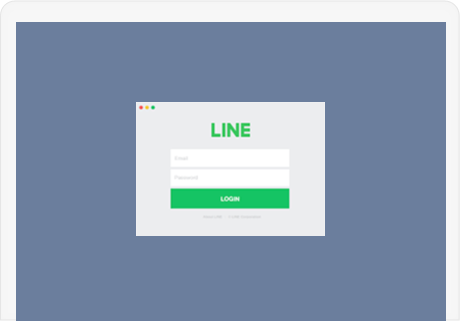
\includegraphics[scale=0.5]{line-login-main-contents.png}  
	\caption[LINE Login]{LINE Login} 
	\label{fig:line-login} 
\end{figure}

LINE Login adalah produk dari LINE yang memungkinkan \textit{developer} membuat aplikasinya menyediakan pilihan login melalui akun LINE. Pengguna aplikasi yang dibuat \textit{developer} tidak perlu mendaftar menggunakan email dan password. Login menjadi lebih mudah dan cepat. LINE menyediakan LINE SDK untuk mengintegrasikan LINE Login dengan native apps.

\subsection{LINE Bot Designer}

\begin{figure}[H]
	\centering  
	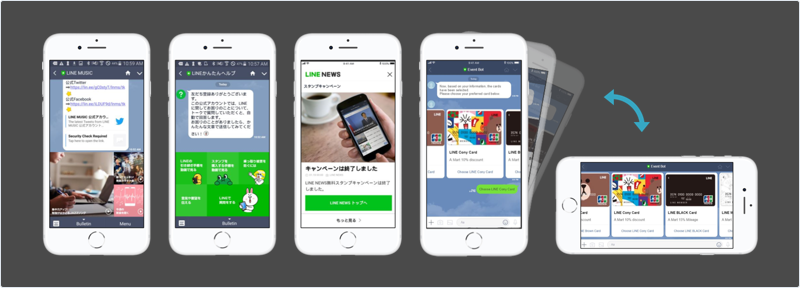
\includegraphics[scale=0.5]{bot-designer.png}  
	\caption[LINE Bot Designer]{LINE Bot Designer} 
	\label{fig:bot-designer} 
\end{figure}

LINE Bot Designer (Gambar~\ref{fig:bot-designer}) adalah produk LINE yang memungkinkan \textit{developer} membuat prototipe LINE bot lebih cepat dan lebih mudah tanpa mengetahui pemrograman. Dengan produk ini, \textit{developer} dapat mendesain chatbots sesuai skenario yang diinginkan.

\subsection{Clova}

\begin{figure}[H]
	\centering  
	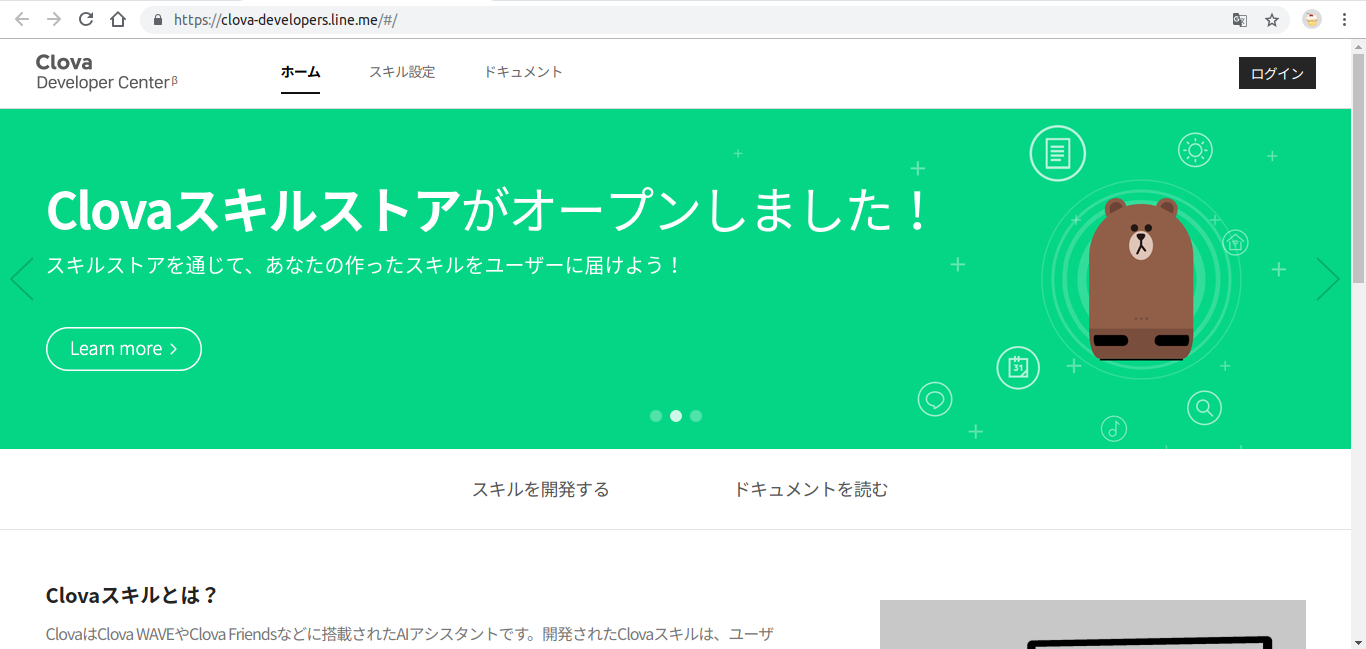
\includegraphics[width=\textwidth]{clova_site.png}  
	\caption[Situs web Clova]{Situs web Clova (https://clova-developers.line.me)} 
	\label{fig:clova_site} 
\end{figure}

Clova adalah sebuah AI Assistant (aplikasi dengan kecerdasan buatan yang berfungsi sebagai asisten) yang dipasang di dalam Clova Wave dan Clova Friends. Clova masih dalam tahap \textit{developer}an dan (pada saat skripsi ini dibuat) tersedia dalam versi beta. Tidak ada dokumentasi resmi untuk produk ini, namun disediakan situs web untuk menggali informasi tentang Clova : https://clova-developers.line.me (Gambar~\ref{fig:clova_site}). Pada saat skripsi ini ditulis, situs web ini hanya tersedia dalam bahasa Jepang sehingga membutuhkan penerjemah apabila tidak menguasai bahasa Jepang.

\subsection{LINE Pay}
\begin{figure}[H]
	\centering  
	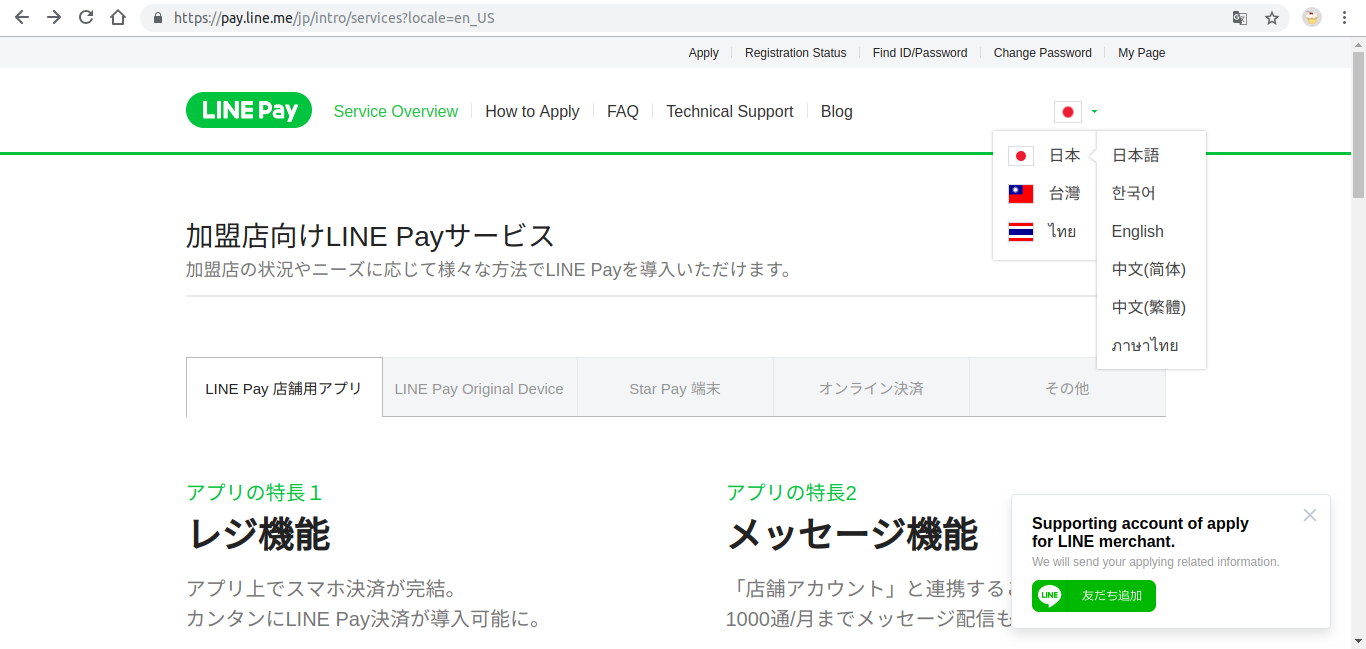
\includegraphics[width=\textwidth]{line_pay_site.png}  
	\caption[Situs web LINE Pay]{Situs web LINE Pay (https://pay.line.me)} 
	\label{fig:line_pay_site} 
\end{figure}

LINE Pay adalah produk LINE yang memungkinkan \textit{developer} mengintegrasikan aplikasi yang dibuat \textit{developer} dengan fitur pembayaran melalui LINE Pay. Pada saat skripsi ini dibuat, tidak ada dokumentasi resmi untuk mengintegrasikan LINE Pay dengan aplikasi yang \textit{developer} buat. Namun, \textit{developer} dapat menggali informasi tentang fitur LINE Pay di situs https://pay.line.me (Gambar~\ref{fig:line_pay_site}). Situs ini menyediakan informasi LINE Pay di negara Jepang, Republik Tiongkok / Taiwan, dan Thailand. Situs ini tersedia dalam bahasa Jepang, Korea, Inggris, China dengan aksara sederhana, China dengan aksara tradisional, dan Thailand.

\subsection{Messaging API } 
\begin{figure}[H]
	\centering  
	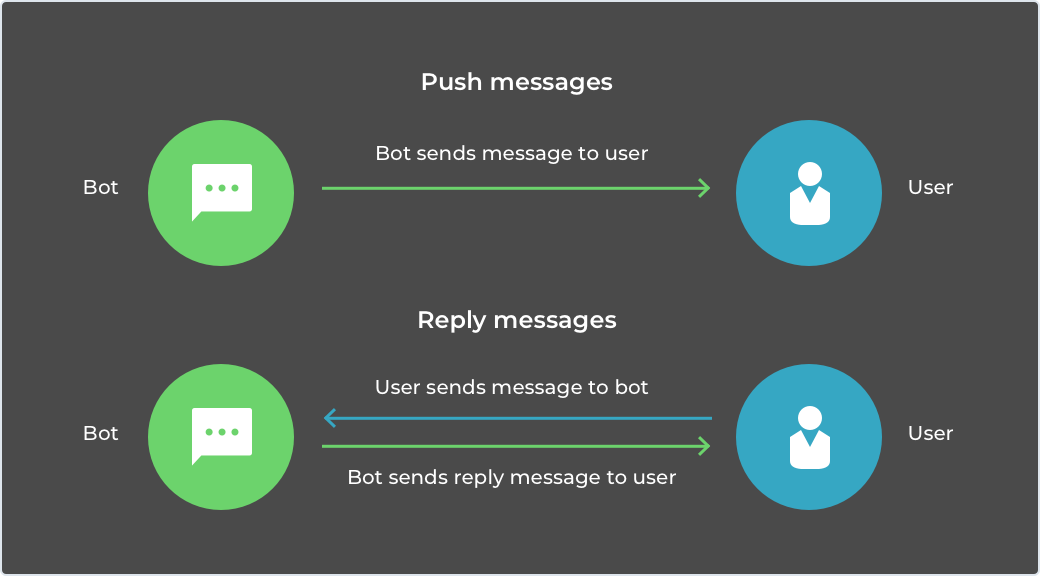
\includegraphics[width=\textwidth]{messaging-api-push-reply-message.png}  
	\caption[Push message dan reply message pada Messaging API]{Messaging API memungkinkan \textit{developer} mengirim push message dan reply message} 
	\label{fig:messaging-api-push-reply-message} 
\end{figure}

Messaging API adalah produk LINE yang memungkinkan \textit{developer} untuk membangun bot sebagai sarana komunikasi dua arah antara layanan yang dibangun \textit{developer} dengan pengguna LINE. Dengan Messaging API, \textit{developer} dapat mengirimkan push message dan reply message (Gambar~\ref{fig:messaging-api-push-reply-message}) ke akun LINE@. Push message adalah pesan yang bot kirimkan ke pengguna LINE. Reply message adalah pesan yang bot kirimkan untuk membalas pesan dari pengguna LINE.

Line Menyediakan Messaging API untuk membangun messaging bot. Messaging API memungkinkan data dioper antara server dari aplikasi bot dengan LINE Platform. Ketika pengguna Line mengirimkan pesan ke bot, sebuah webhook akan terpicu dan LINE Platform akan mengirimkan permintaan ke URL webhook bot. Server akan mengirim permintaan ke LINE Platform untuk merespon pengguna. Permintaan akan dikirimkan dalam format JSON. Arsitektur dari Messaging API dapat dilihat pada Gambar~\ref{fig:messaging_api_architecture}.

\begin{figure}[H]
	\centering  
	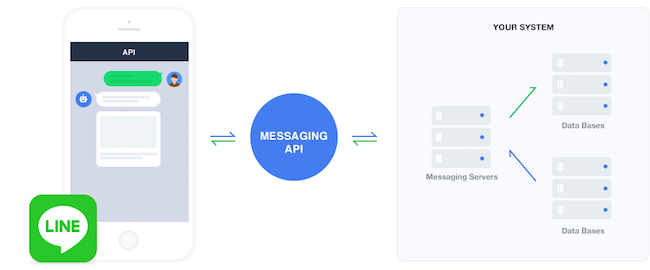
\includegraphics[width=\textwidth]{messaging-api-architecture.png}  
	\caption[Arsitektur Messaging API]{Arsitektur Messaging API} 
	\label{fig:messaging_api_architecture} 
\end{figure}

\textit{Developer} dapat melakukan hal-hal berikut dengan Messaging API :
\begin{itemize}
\item Mengirimkan reply message
\item Mengirimkan push message
\item Mengirimkan berbagai jenis pesan
\item Mendapatkan profil pengguna yang berinteraksi dengan bot
\item Bergabung dengan percakapan grup /group chats
\end{itemize}

Untuk menggunakan Messaging API, \textit{developer} memerlukan akun LINE@. Messaging API juga dapat digunakan menggunakan akun resmi/\textit{official accounts}. Akun resmi mendapatkan fitur tambahan untuk pengguna enterprise.

\subsubsection{Membuat Channel}
Untuk memulai membangun bot dengan Messaging API, \textit{developer} perlu membuat channel terlebih dahulu. Channel adalah penyambung antara LINE platform dan aplikasi yang dibuat \textit{developer}. Berikut langkah-langkah untuk membuat channel :
\begin{enumerate}
\item Langkah ke-1 : Masuk ke LINE Developers console

\begin{figure}[H]
	\centering  
	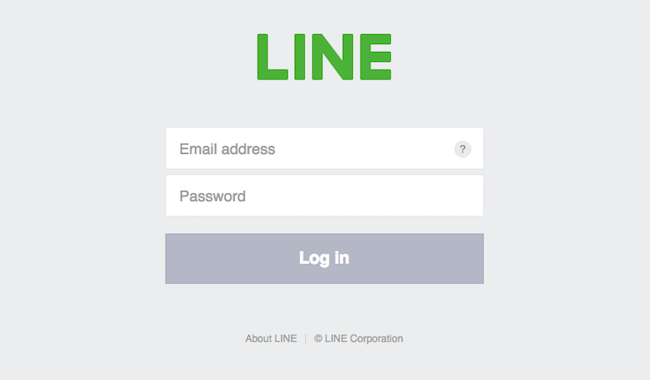
\includegraphics[width=\textwidth]{line-developers-console-login.png}  
	\caption[Tampilan LINE developer console saat login]{Tampilan LINE developer console saat login} 
	\label{fig:line-developers-console-login} 
\end{figure}

\textit{Developer} perlu masuk ke LINE Developers console (https://developers.line.me/en/) dengan alamat email dan password dari akun LINE \textit{developer} (Gambar~\ref{fig:line-developers-console-login}). Jika \textit{developer} belum memiliki akun LINE, \textit{developer} perlu mengunduh aplikasi LINE untuk mendaftar akun LINE.

\item Langkah ke-2 : Mendaftar sebagai developer (\textit{developer})

\begin{figure}[H]
	\centering  
	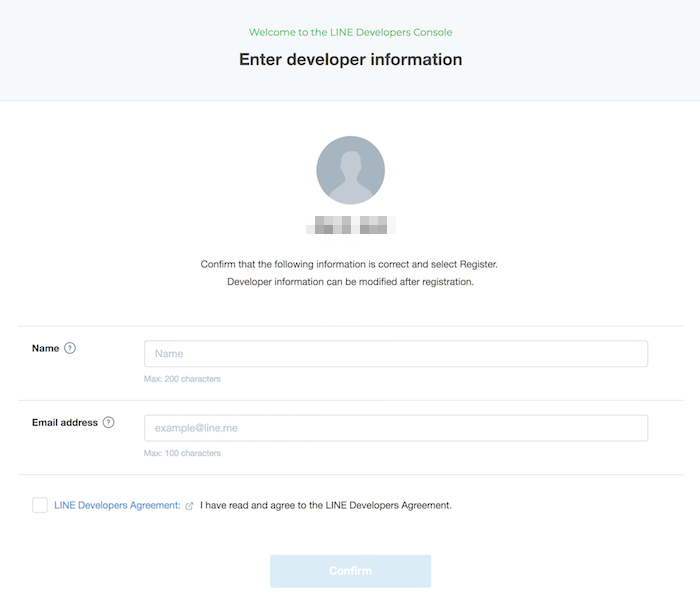
\includegraphics[width=\textwidth]{line-developers-console-register-developer.png}  
	\caption[Tampilan LINE developer console saat register developer]{Tampilan LINE developer console saat register developer} 
	\label{fig:line-developers-console-register-developer} 
\end{figure}

Apabila \textit{developer} baru pertama kali masuk ke LINE Developers console, \textit{developer} perlu membuat akun developer (Gambar~\ref{fig:line-developers-console-register-developer}). \textit{Developer} hanya perlu mencantumkan nama dan alamat email untuk mendaftar.

\item Langkah ke-3 : Membuat provider baru

Provider adalah individu atau perusahaan yang menyediakan aplikasi yang akan dibuat. \textit{Developer} perlu mencantumkan nama provider untuk membuat provider baru. \textit{Developer} dapat menuliskan nama \textit{developer} sendiri atau nama perusahaan \textit{developer}.

\item Langkah ke-4 : Membuat channel
\begin{figure}[H]
	\centering  
	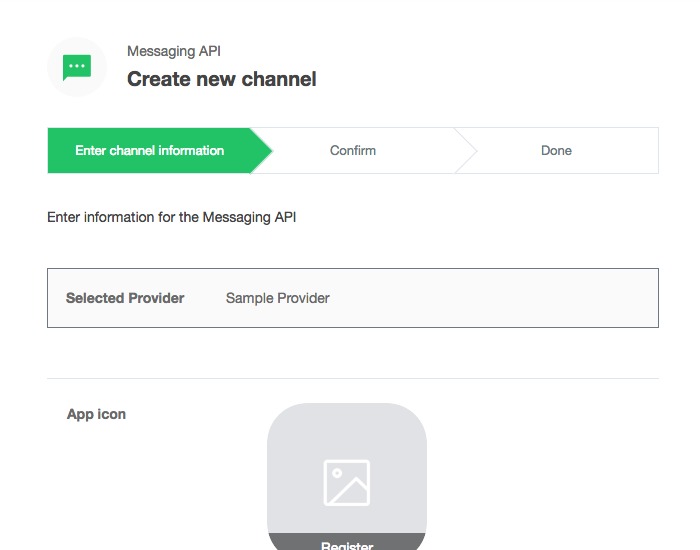
\includegraphics[width=\textwidth]{line-developers-console-create-channel.png}  
	\caption[Tampilan LINE developer console saat membuat channel]{Tampilan LINE developer console saat membuat channel} 
	\label{fig:line-developers-console-create-channel} 
\end{figure}

\textit{Developer} perlu memasukkan informasi yang dibutuhkan untuk membuat channel :
\begin{itemize}
\item Ikon aplikasi

Dokumen gambar untuk ikon aplikasi harus dibawah 3MB dengan ekstensi JPEG/PNG/GIF/BMP.

\item Nama aplikasi

Nama aplikasi tidak boleh lebih dari 20 karakter. Kata "LINE" tidak dapat digunakan sebagai nama aplikasi, walaupun kapitalisasinya tidak sama. Setelah dikonfirmasi, nama aplikasi tidak dapat diubah untuk tujuh hari ke depan.

\item Deskripsi aplikasi

Deskripsi aplikasi tidak boleh lebih dari 500 karakter.

\item Plan

Terdapat dua pilihan, Developer Trial dan Free. Plan Developer Trial memungkinkan \textit{developer} untuk membuat bot yang dapat mengirimkan push message dan memiliki 50 teman. Apabila \textit{developer} memilih plan ini, maka \textit{developer} tidak dapat melakukan upgrade atau membeli ID premium. Plan Free memungkinkan \textit{developer} untuk membuat bot dengan jumlah teman tak terbatas, namun \textit{developer} tidak dapat mengirimkan push message. \textit{Developer} dapat melakukan upgrade kapan saja dengan plan ini.

\item Kategori dan Subkategori

\textit{Developer} dapat memilih kategori dan subkategori yang cocok dengan aplikasi yang sedang dikembangkan.

\item Alamat email

Alamat email yang dicantumkan adalah alamat email yang akan menerima notifikasi dan pengumuman penting dari LINE. Maksimal karakter pada alamat email adalah 100 karakter.

\end{itemize}

\item Konfirmasi
\begin{figure}[H]
	\centering  
	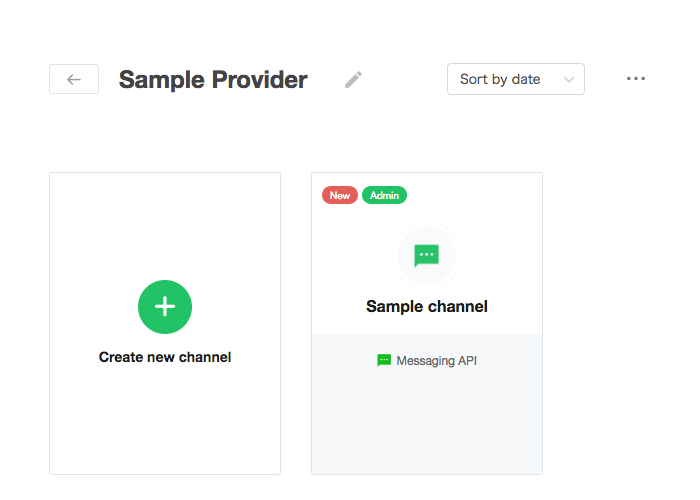
\includegraphics[width=\textwidth]{line-developers-console-confirm-channel.png}  
	\caption[Tampilan LINE developer console saat konfirmasi pembuatan channel]{Tampilan LINE developer console saat konfirmasi pembuatan channel} 
	\label{fig:line-developers-console-confirm-channel} 
\end{figure}

Konfirmasi channel yang baru saja dibuat.

\end{enumerate}


\subsubsection{Membuat bot}
Setelah membangun channel, \textit{developer} perlu menyiapkan server untuk menjadi host dari bot. \textit{Developer} dapat menggunakan layanan cloud platform, seperti Heroku. Setelah itu, \textit{developer} dapat mulai mengatur bot pada console.

Aplikasi bot membutuhkan channel access token untuk membuat API call dan webhook URL untuk menerima webhook payload dari LINE Platform. Channel access token adalah long-lived token (token yang tidak memiliki kadaluarsa) yang harus diatur di dalam authorization header ketika membuat API call. \textit{Developer} dapat menerbitkan lagi channel access token kapanpun melalui console. Untuk menerbitkan channel access token, klik Issue pada "Channel settings" di halaman console. Sedangkan webhook URL adalah titik akhir dari server aplikasi bot dimana webhook payload dikirimkan.

Untuk mengatur webhook URL, \textit{developer} dapat memasukkannya ke halaman Channel settings pada console. Webhooks harus diaktifkan terlebih dahulu dengan menekan tombol enable webhooks. Untuk memeriksa apakah webhook URL dapat menerima event webhook, tekan tombol Verify dan pastikan hasilnya "Success". Webhook URL harus menggunakan HTTPS dan memiliki sertifikat SSL yang diterbitkan oleh certificate authority (CA) yang terotorisasi.

Setelah token dan webhook URL berhasil diset, tambahkan bot sebagai teman melalui akun LINE. \textit{Developer} dapat melakukannya dengan scan kode QR pada Channel Settings.

\subsubsection{Menkonfigurasi Keamanan}
\textit{Developer} dapat mengkonfigurasi keamanan tapi tidak wajib dilakukan. Untuk meningkatkan keamanan, \textit{developer} dapat mengatur server yang dapat memanggil API pada LINE Platform pada Security settings. \textit{Developer} dapat mendaftarkan alamat IP secara individual atau jika \textit{developer} memiliki server yang banyak \textit{developer} dapat menggunakan notasi classless inter-domain routing (CIDR) untuk mendaftarkan alamat jaringan.

\subsubsection{Alur kerja Messaging API}
Ketika user berinteraksi dengan bot seperti mengirimkan pesan atau menambah bot sebagai teman, LINE Platform mengirimkan HTTP POST request yang berisi webhook event object ke bot server yang disebutkan di kolom "Webhook URL" pada console. Request header berisi signature. 

Untuk mengecek apakah server dapat menerima webhook event, blok bot pada LINE dan cek server logs untuk menkorfimasi bahwa server dapat menerima unfollow event dari LINE Platform.

Untuk memastikan request yang dikirim berasal dari LINE Platform, bot server harus memvalidasi X-Line-Signature pada request header. Caranya dengan :
1. Menggunakan channel secret sebagai secret key, mengenerate Base64-encoded digest dari request body menggunakan algoritma HMAC-SHA256
2. Menkonfirmasi signature X-Line-Signature dalam request header cocok dengan digest.
 

\subsubsection{Webhook Event Object}
\begin{enumerate}
\item Khusus untuk one-on-one chat

\begin{itemize}
\item Message Event

Menunjukkan bahwa ada user yang mengirim pesan. Event ini dapat dibalas.

\item Follow Event

Menunjukkan bahwa akun bot ditambahkan sebagai teman (atau unblocked). Event ini dapat dibalas.

\item Unfollow Event

Menunjukkan bahwa akun bot diblok

\item Postback event

Menunjukkan user melakukan aksi postback. Event ini dapat dibalas.

\item Beacon event

Menunjukkan bahwa user telah masuk atau keluar dari jangkauan LINE Beacon. Event ini dapat dibalas.

\item Account link event 

Menunjukkan bahwa user telah melink akun LINE dengan akun layanan \textit{developer}. 

\end{itemize}

\item Group chats

\begin{itemize}
\item Message event

Menunjukkan bahwa ada user yang mengirim pesan. Event ini dapat dibalas.

\item Join event

Menunjukkan bot telah bergabung ke sebuah group chat

\item Leave event

Menunjukkan bot telah keluar dari sebuah group chat

\item Postback event

Menunjukkan user melakukan aksi postback. Event ini dapat dibalas.

\end{itemize}

\end{enumerate}

\subsubsection{Operasi pada bot}
\textit{Developer} dapat melakukan operasi berikut lewat bot :
\begin{enumerate}
\item Mengirim reply message

Reply message adalah pesan yang dikirim sebagai respons dari user-generated event. User-generated event adalah event yang muncul karena user berinteraksi dengan bot, misalnya mengirim pesan. \textit{Developer} hanya dapat membalas webhook events yang memiliki reply token.
Untuk membalas pesan, kirim HTTP POST request ke /bot/message/reply. Sertakan channel access token di dalam authorization header dan reply token di request body. \textit{Developer} dapat mengirimkan sampai 5 message object per request.

\item Mengirim push message

Untuk mengirim push message, \textit{developer} harus memerhatikan plan yang dipakai. Apabila \textit{developer} memakai plan Free maka \textit{developer} tidak dapat melakukan operasi ini. Push message adalah pesan yang dapat bot kirimkan ke user kapanpun. Push message tidak membutuhkan reply token seperti saat mengirim reply message. Ketika mengirim push message, sebutkan user ID di dalam property to. ID penerima dapat ditemukan dari webhook event object. Apabila penerima hanya satu, kirimkan request ke /bot/message/push. Sedangkan apabila penerima ada beberapa, kirimkan ke /bot/message/multicast. \textit{Developer} dapat mengirimkan sampai 5 message object per request.

\item Mendapatkan konten yang dikirim oleh user

Untuk mengambil gambar, video, atau audio yang dikirim user, kirimkan HTTP GET request ke /bot/message/{messageId}/content. Konten yang dikirim oleh user otomatis dihapus dalam jangka waktu tertentu.

\item Mendapatkan informasi user profile

Untuk mendapatkan informasi user profile dari user yang menambahkan bot atau mengirim pesan ke bot, kirimkan HTTP GET request ke /bot/profile/{userId}. Request ini akan mengembalikan display name, user ID, profile image URL, dan status message (jika tersedia) dari user.
\end{enumerate}

\subsection{LINE@ Manager}
LINE@ Manager adalah alat untuk mengatur akun LINE@ (LINE bot). \textit{Developer} dapat meningkatkan user experience dengan mengatur halaman akun, membuat Timeline post, dan menggunakan fitur lain yang disediakan LINE@ Manager. Berikut adalah hal-hal yang bisa dilakukan :
\begin{enumerate}
\item Mengubah tampilan halaman akun

\textit{Developer} dapat mengubah gambar cover, logo, tombol, dan informasi yang disediakan

\item Mengatur greeting message

Jika \textit{developer} mengaktifkan Greeting message pada Channel settings, maka \textit{developer} dapat mengatur greeting message yang akan dikirim ke user saat pertama kali menambahkan bot sebagai teman. \textit{Developer} dapat melakukannya juga dengan program melalui follow webhook event.

\item Mengatur auto reply message

Jika \textit{developer} mengaktifkan "Auto reply message" pada Channel settings, maka \textit{developer} dapat mengatur pesan balasan otomatis setiap user mengirimkan pesan ke bot.
\end{enumerate}